\chapter{Machine Learning}
\label{c3:intro}

\thispagestyle{empty}
\epigraph{\itshape ``Learn everything about something, and something about everything''}
{---Donald Knuth}

\section{Artificial Intelligence}

Undeniably the term of intelligence has gathered the attention of the most philosophical studies and discussions whether is something that exclusively exist in humans and animal or that it can be reproducible. If the latter is valid, how can we encode the human cognition in order to be understandable from a machine? Does it happen by simulating a small children's brain or let it learn by itself~\cite{turing1950computing}?
With the exponential growth of computational power the interest for automating certain procedures has increased. An effort to develop intelligent systems has assisted to create such applications that can aid to decision making in certain tasks. The term of \textit{Artificial Intelligence} has been established by $1956$ and some of the most remarkable real world applications are image recognition, natural language processing, driving assistance, art generation etc., have developed from self-trained systems without human interference. That particular domain of AI is called Machine Learning.


\section{Machine Learning}
\label{c3:ml}
In the era of big data we are surrounded of unlimited amounts of new data, generated each second. Billions of images from popular platforms like Instagram, Flickr and Unsplash to hundred of thousand hours of uploaded video, millions of eretail transactions per hour and so on.
This burst of data are subject to ubiquitous methods of data analysis which derive from machine learning techniques.
Machine learning, at its definition is a set of applied statistical methodologies that can learn from data upon a specific task and automatically discover patterns or learn to map data on some class.

Intuitively we take advantage of this knowledge to predict a pattern of unknown data or conduct inference by generating new information~\cite{murphy2012machine}.
Pattern recognition is linked with the automatic discovery of recurrences in data through the use of computer algorithms. The produced knowledge can assist to take actions, such decision making or classify data to different categories~\cite{bishop2006pattern}.

A more formal definition of Machine Learning is the following:
\begin{itemize}
 \item A \textit{computer program}, is a suitable to the task algorithm that has the capability of training.
 \item Experience \textit{E}, is the data set, that the algorithm is trained.
 \item The task \textit{T}, that the algorithm will learn to solve.
 \item The performance \textit{P}, the measurement that will be used in order to monitor the algorithm on how well performs on the task.
\end{itemize}


\subsection{Learning Tasks}

Machine learning diverges from the classical rule-based approach of an algorithm which is a standard procedure that one can explicitly define. On the other hand, an ML algorithm is not an algorithmic process but a set of methods that are not programmed but trained on sets of data.

Most of ML methods, fall into 3 broad categories:
\begin{itemize}
 \item \textbf{Supervised Learning}, the algorithm is trained on associations of the input data to  corresponded labels.
 \item \textbf{Unsupervised Learning}, the algorithm is trained without human supervision.
 \item \textbf{Reinforcement Learning}, a less commonly used type of learning which works as a rewarding/punishing system upon an actor~\cite{sutton2018reinforcement}, but is beyond the scope of this work.
\end{itemize}

In this thesis, we focus on supervised learning to solve a non-trivial task, in the context of image aesthetics.

To begin with, consider the example of handwritten digit recognition illustrated in Figure~\ref{c3:mnist}. Each digit is represented by a 28 $\times$ 28 pixel gray-scale image and so it can represented by a 1-d vector $x$ of 784 size. The task is to build a model that will take as input such a vector $x$ and will produce a label identified by the digit number 0,\dots,9 to the output.

\begin{figure}[h!]
    \centering  
    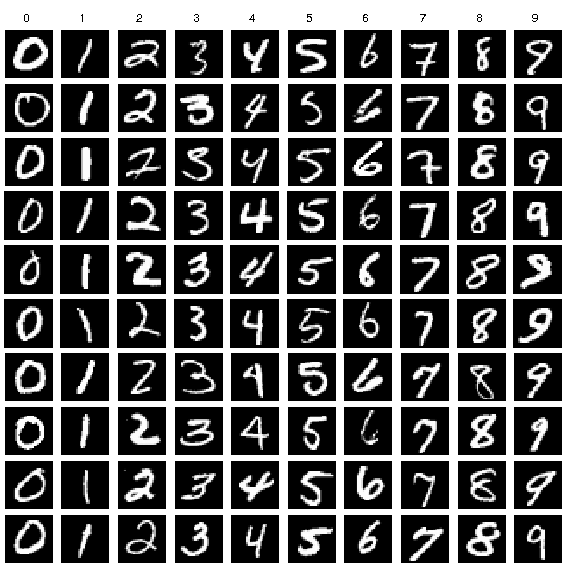
\includegraphics[width=.4\textwidth]{figures/chap3/ml/mnist}
    \caption{Hand-written digits data set}
    \label{c3:mnist}
\end{figure}

The task is non trivial at hand due to the variety of handwritten digits and employing a rule-based solution using handcrafted rules and classical image processing techniques will lead to an explosive amount of rules and so forth will give poor results.
By adopting a machine learning approach, we can create a large set of $N$ digits namely a \textit{training set}, of samples $X = \{x_1,\dots,x_N \}$ and target vectors $y = \{y_1,\dots,y_N \}$ and use it to train an adaptive model by optimizing each parameters in order to maximize classification performance.
Typically we are feeding the machine learning model with pairs of:
\begin{enumerate}
 \item \textbf{samples} $x$ expressed by the digit vector and 
 \item \textbf{target} vectors $t$, which represent the identity of the corresponded digit
\end{enumerate}

A target vector, denoted as \textbf{label}, is produced from a human input, known as annotation process.
During the \textit{training phase} model is determined to learn the \textit{training data}.

More specifically, it learns to map the samples on the associated targets and by the end of training it is expected to identify unknown samples which hasn't seen before, namely, the \textit{test} set. The ability to recognize an unknown digit falls to the problem of \textit{generalization}~\cite{mitchell1986explanation} which is a practical problem in all applications.
For the most applications, input samples are subject to typical \textit{preprocessing} steps in order to transform them into a new parameter space to ease and accelerate training and learning. For example in the case of hand written images, a gray-scale image is represented in 8-bit ranges from 0-255 integer values. Rescaling the values into 0-1 scale, will help to reduce the variability of the data it make it much easier for the classifier to distinguish between the classes. The preprocessing stage can be sometimes called \textit{feature extraction}.
In most of the tasks, where the raw data are multi and high dimensional, preprocessing step is essential, otherwise it will be computationally infeasible for the machine learning model to converge.
Such tasks as the one described above fall into the domain of \textbf{supervised learning} problems and belong to a broader family of problems those, of \textit{Image Classification}. In such a task a model \textit{g} also called \textit{estimator}, will be trained and learn to map an input vector sample, to a certain class, from a finite number of available classes $x_i \rightarrow y_i$.

Practically, a perfect association can never be made, because of the model's incapability to describe complicated mappings or due to the descriptive information of the features. Thus, we state that a model \textit{g} \textbf{predicts} or \textbf{infers} hypothesis $\hat{y}_i$ for the sample $x_i$, as $\hat{y}_i = g(x_i)$.

On the other hand assuming that the desired output could be a continuous variable, the task is called \textit{regression}. An example of regression problem could be the prediction of a house price given an input feature vector that represents e.g. a residential area, size of house etc.

In many cases where the human input and target labels are unavailable, the training data consist only of a set of input samples \textbf{x}. Such problems belong to the category of instance-based learning or \textit{unsupervised learning}. Such tasks can be \textit{clustering} where the algorithm discovers groups of similar instances within the training samples or to determine the distribution of data and discover latent representations from high dimensional input projected to a smaller number of dimensions for the purpose of \textit{visualisation}. An example of a visualised clustering application on the same data set is illustrated in Figure~\ref{c3:clustering}.

\begin{figure}[h!]
    \centering  
    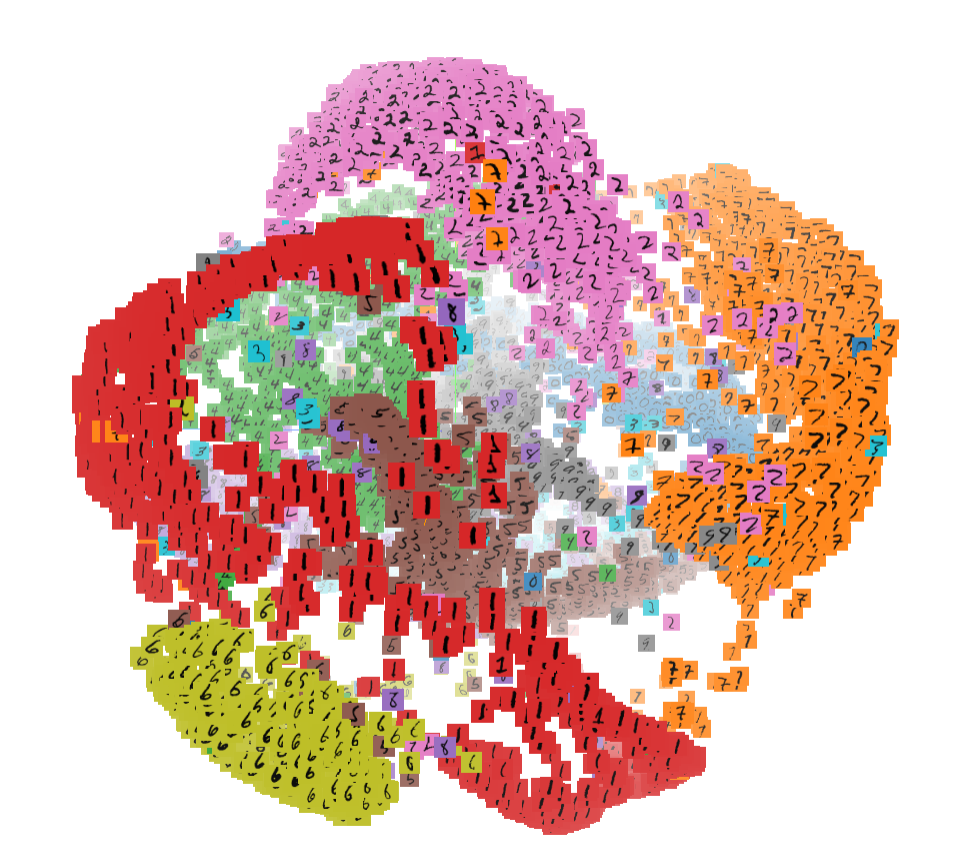
\includegraphics[width=.5\textwidth]{figures/chap3/ml/clusters}
    \caption{Hand-written digits data set visualised in clusters}
    \label{c3:clustering}
\end{figure}

\section{Deep Learning}

A sub-domain of machine learning, known as Deep Learning (DL), has substantial growth in many types of machine learning systems over the latest years. Conventional machine learning techniques are limited to their ability to process the data at its natural form~\cite{lecun2015deep}. Machine learning systems are relying to careful feature engineering and sophisticated feature extraction techniques with considerable domain expertise, in order to feed a classifier with data and produce a result.
Deep learning methods are representation learning methods able to fed with unstructured data (images, text, voice, etc.) without any prior handcrafted feature extraction technique. It utilises of non-linear activated modules able to transform the data directly from the input, into high-level feature representations. Compositing multiple modules we are able to learn very complex functions due to the hierarchical structure of the network. A deep neural network is illustrated in Figure~\ref{c3:dl}.

\begin{figure}[h!]
    \centering  
    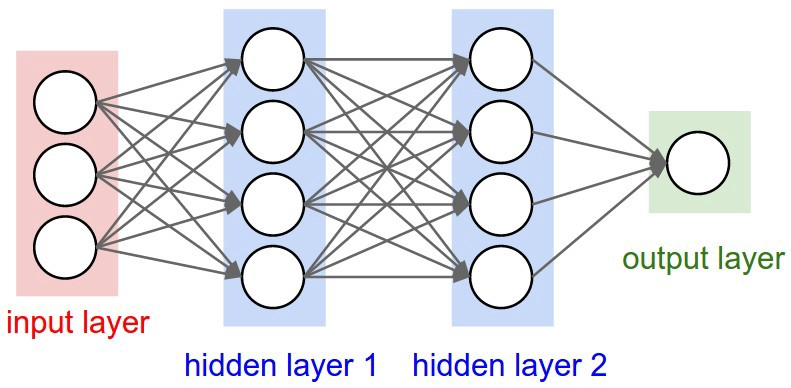
\includegraphics[width=.6\textwidth]{figures/chap3/ml/dl}
    \caption{Deep neural network}
    \label{c3:dl}
\end{figure}

This has led to groundbreaking advances in the domain of \textit{Computer Vision} and \textit{Natural Language Processing} as one is able to process huge amounts of data and solve complicated problems that were unable to get solved by the AI community for many years.

Deep learning turned out to be very good at discovering complex structure in high-dimensional data and consequently deep learning models are successfully deployed and support real life applications in domains of science and business products.

\section{Computer Vision}

From the early 70s the field of computer vision started as an attempt to shed some light in the open problem of visual perception. Pioneers of their time such Winston~\cite{winston1975psychology} attempted to set a frame on the global scene understanding, Barrow~\cite{barrow1981interpreting}, proposed an approach to understand the fundamental importance of surface perception interpreting line drawing and Marr~\cite{marr1982vision} as discussed in Section~\ref{c2:aesthetics}, introduced the notion of a visual processing system summarised in the three levels of computational theory, representation and algorithms and hardware implementation.
In 80s, more sophisticated techniques have emerged to perform quantitative image and scene analysis for better edge and contour detection Canny~\cite{canny1986computational}.
In 1990s, a burst in more integrated applications was recorded such in image segmentation by Haralinck~\cite{haralick1985image} and in image restoration by Banham~\cite{banham1997digital}.
In the decade of 2000, the exponential growth in computational photography increased the demand for computational techniques for the every day photography. For example image stitching~\cite{brown2007automatic} to create photographic panoramas, automatic exposure bracketing into a composition of high dynamic range scene~\cite{reinhard2010high}, tone mapping to effectively correct the image gamut and prevent from burned or darken images~\cite{durand2002fast}, super resolution and blur removal~\cite{baker2002limits}, vignette and exposure calibration~\cite{goldman2010vignette}.

The problem we are going to tackle in this work, lies in the domain of computer vision (CV). Computer vision tries to describe the natural world in images and reconstruct its properties, such shape, illumination and colour distributions~\cite{szeliski2010computer}.

Nowadays, we are interacting with computer vision applications to a wide variety of solved problems such medical imaging, optical character recognition (OCR), pose estimation, photogrammetry, motion capture, face and object detection, image stitching, image filtering and many more.

\begin{figure}[h!]
    \centering  
    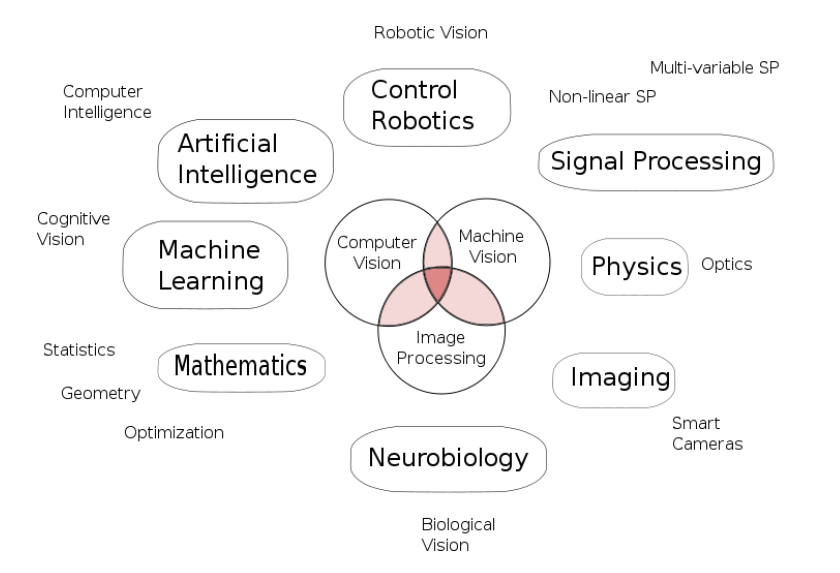
\includegraphics[width=.6\textwidth]{figures/chap3/cv/cv}
    \caption{Computer vision map}
    \label{c3:cv}
\end{figure}

\begin{figure}[ht!]
    \centering  
    \subfigure[]{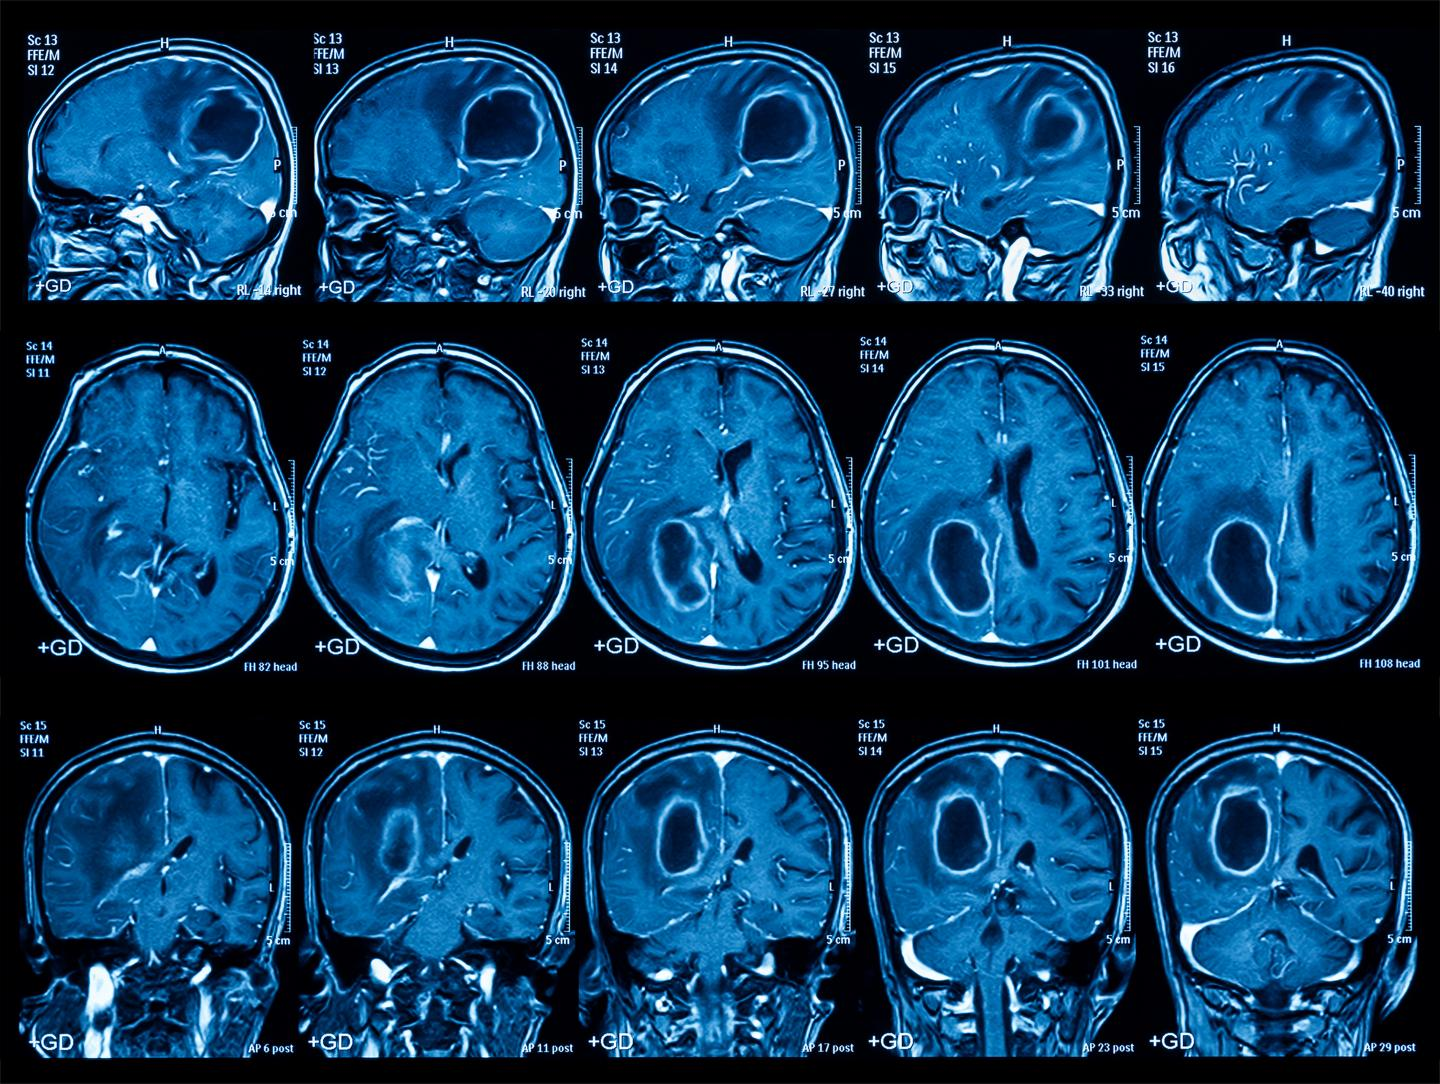
\includegraphics[width=.3\textwidth]{figures/chap3/cv/medical}}
    \subfigure[]{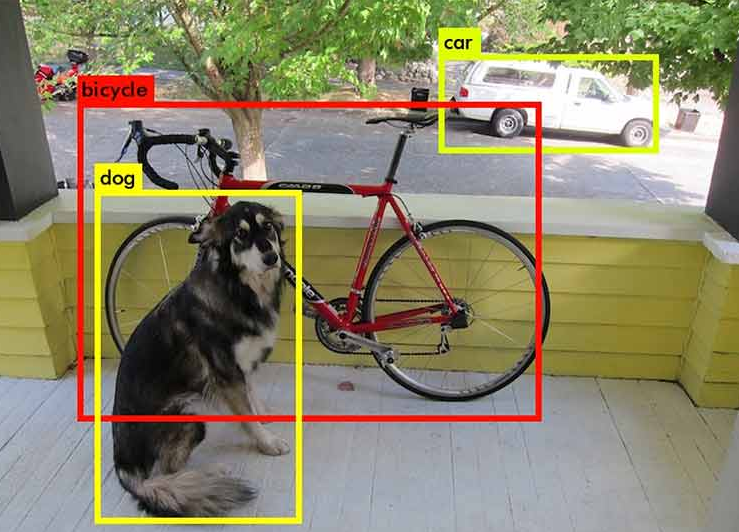
\includegraphics[width=.3\textwidth]{figures/chap3/cv/od}}
    \subfigure[]{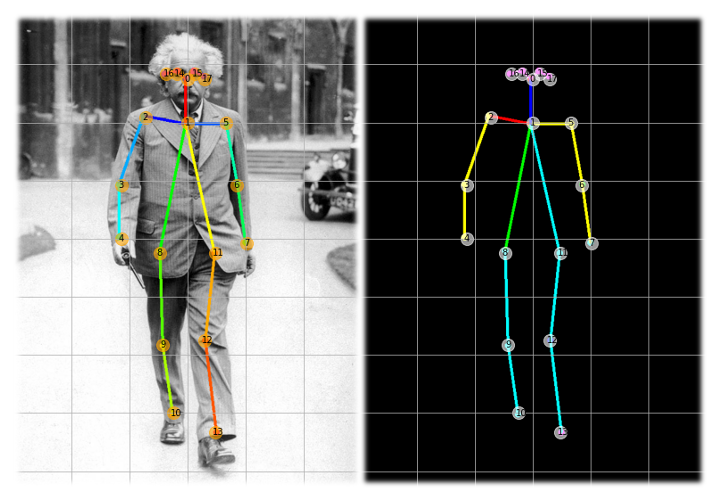
\includegraphics[width=.3\textwidth]{figures/chap3/cv/pose}}
    \subfigure[]{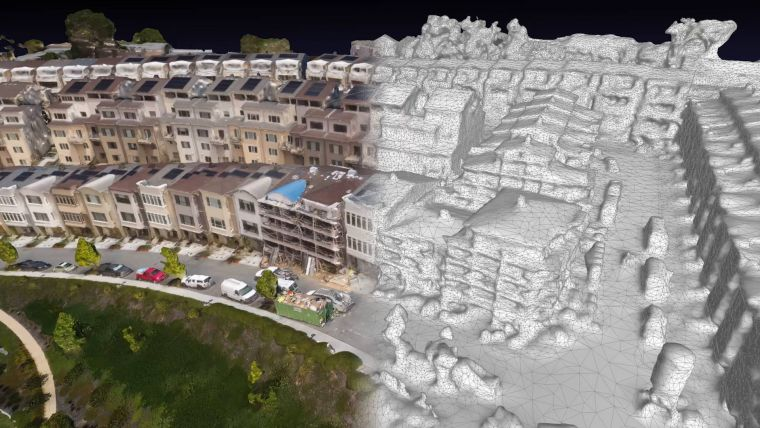
\includegraphics[width=.4\textwidth]{figures/chap3/cv/photogrametry}}
    \subfigure[]{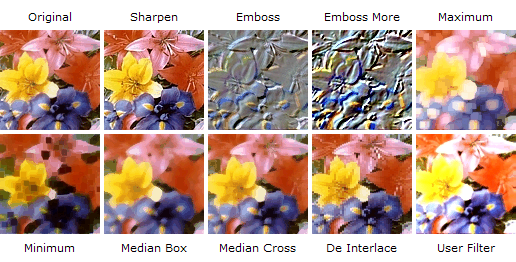
\includegraphics[width=.5\textwidth]{figures/chap3/cv/filters}}
    \caption{Computer vision applications: (a) Medical imaging, (b) object detection, (c) Pose estimation, (d) Photogrametry, (e) Image filtering}
    \label{c3:cv_apps}
\end{figure}

\section{Neural Networks}

Neural networks (NN) is a type of model that can be utilised to solve efficiently classification problems. The basic building unit that constructs a neural network is called \textit{Neuron} or \textit{Perceptron}~\cite{rosenblatt1958perceptron}.

A neuron is able to perform two operations: a linear (or affine) transformation to its input and a non-linear function application to the output. A neuron is described from the next equation:
\begin{ceqn}
\label{c3:perceptron_eq}
\begin{align}
    z = f(w \cdot x + b)
\end{align}
\end{ceqn}
In the above equation~\ref{c3:perceptron_eq}, the input is represented as a vector $x \in \mathbb{R}$ such as an image or audio. This input is multiplied by the weight matrix $w \in \mathbb{R}$ which coefficient is a tunable parameter bias $b \in \mathbb{R}$.
These operations consist the linear transformation of the Perceptron. 
Then, every component of the result vector is passed through a non-linear function \textit{f} which is called \textit{activation function}.
The most popular activation functions that are used thoroughly are the sigmoid, tanh, ReLU and softmax. More for the activation functions is discussed in Section~\ref{c3:activation_functions_sec}.

When we say that a network learns, it means that in the training phase the neuron parameters \textit{w} and \textit{b} are being adapted in respect of the network output. A neuron is presented in Figure~\ref{c3:perceptron}.

\begin{figure}[h!]
    \centering  
    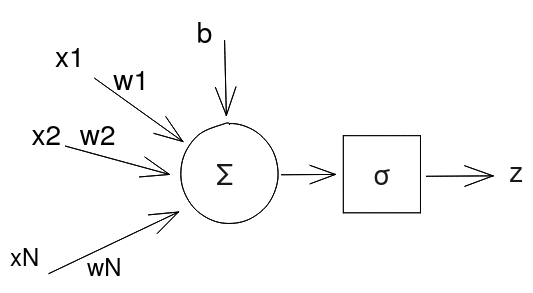
\includegraphics[width=.5\textwidth]{figures/chap3/ml/neuron}
    \caption{A representation of a neuron. N number of \textit{x} input vectors are multiplied with the corresponded weights \textit{w} with added bias constant \textit{b}. The outcome activates a non-linear function.}
    \label{c3:perceptron}
\end{figure}

\subsection{Multi-layer Perceptron}

A typical neural network consists of multiple layers; the output of one is the input of the other in the next layer. In such hierarchical fashion, the network is able to estimate non-linear functions. 
Repeating this process, it becomes a multi-layer percepton (MLP) network as it is shown in Figure~\ref{c3:mlp}.

\begin{figure}[h!]
    \centering  
    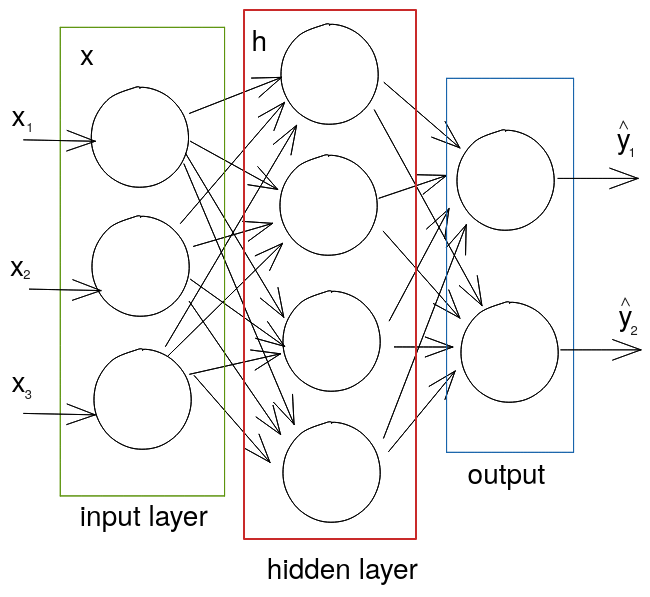
\includegraphics[width=.5\textwidth]{figures/chap3/ml/mlp}
    \caption{A Multi-layer perceptron network having a general feed-forward topology.}
    \label{c3:mlp}
\end{figure}


\section{Training a model}

The standard training procedure applies to any kind of neural network architecture. A simplified case, is a simple shallow network as the above and can be described from the following equation:

\begin{ceqn}
\label{c3:perceptron_mlp_equation}
\begin{align}
    \hat{y} = f(W \cdot x + b),~ W \in \mathbb{R}^{M\times C}, x \in \mathbb{R}^{M}, b \in \mathbb{R}^{C}
\end{align}
\end{ceqn}


Where \textit{M} in the cardinality of input and \textit{C} the number of classes. The input samples constitute a vector of \textit{M} number of values, $x = \{x_{i}^{1}, \dots, x_{i}^{M} \}$
The label value takes the corresponded value of class, as $y_i \in \{ 1, \dots,\text{C} \}$. The output of the network $\hat{y}$ is the one that we are looking for to approach in correspondence to the real label value as it is estimated from the type of activation function in the last output layer.


\subsection{Activation functions}
\label{c3:activation_functions_sec}

Fitting a multilayer neural network requires the choice of an activation function and a network architecture. During the forward pass in training process, the output of a neuron is passed to the next layer only if activated a certain function is applied to the output. While the type of the function is determined from the task to be solved where are going to discuss the activation functions that we have used in our work.
Traditionally in neural networks, sigmoidal activations functions were employed but for a deep neural network (dnn) there is a computational advantage when using a non-sigmoidal rectified linear unit (ReLU)~\cite{schmidt2020nonparametric}.

For classification problems, the ReLU is suggested over a sigmoidal~\cite{glorot2011deep} for image and also text based problems. The ReLU handles better the problematic output of sigmoid function and vanishing gradient phenomenon may occur during the backpropagation. Figure~\ref{c3:activation_functions} illustrates the aforementioned activation functions and the corresponded equation are provided in~\ref{c3:sigmoid_eq},~\ref{c3:relu_eq}.
\begin{ceqn}
\label{c3:sigmoid_eq}
\begin{align}
    \sigma(x) = \frac{1}{1+e^{-x}}
\end{align}
\end{ceqn}

\begin{ceqn}
\label{c3:relu_eq}
\begin{align}
  \text{ReLU}(x) = \text{max}(0,x)
\end{align}
\end{ceqn}

\begin{figure}[ht!]
    \centering  
    \subfigure[]{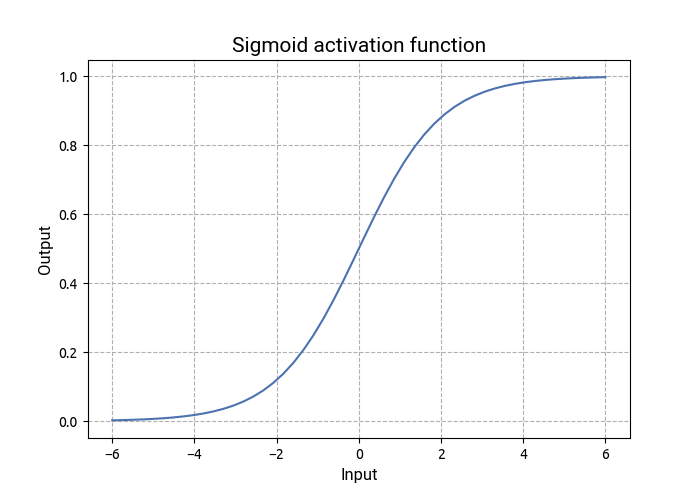
\includegraphics[width=.45\textwidth]{figures/chap3/ml/sigmoid}}
    \subfigure[]{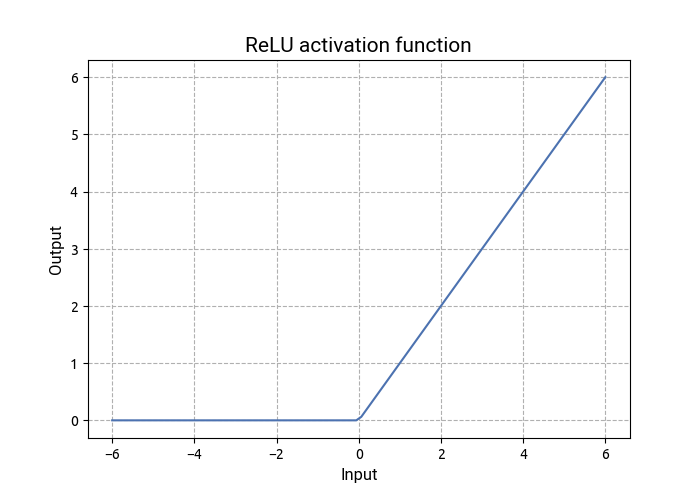
\includegraphics[width=.45\textwidth]{figures/chap3/ml/relu}}
    \caption{Activation functions: (a) Sigmoid, (b) ReLU }
    \label{c3:activation_functions}
\end{figure}

Additionally, concerning the network output the activation function is determined based on the problem at hand. The main problems are the following:

\begin{itemize}
 \item \textbf{Linear Regression}, where the predicted variable has continuous values, so $\hat{y} \in \mathbb{R}$. This task does not require an activation function.
 \item \textbf{Logistic Regression or Classification}, the predicted variable takes a nominal value of the given classes \textit{C}, so $\hat{y} \in \mathbb{N}$. In this case, the \textit{softmax} function is used.
\end{itemize}

Softmax is declared by the equation:

\begin{ceqn}
\label{c3:softmasx_eq}
\begin{align}
  \text{softmax}(z)_i = \frac{e^{z_i}}{\sum_{j=1}^{C} e^{z_j}}
\end{align}
\end{ceqn}

Intuitively, softmax normalize the \textit{z} input into a probability distribution that each output is a posterior probability given a value in the interval $[0,1]$.

\begin{figure}[h!]
    \centering  
    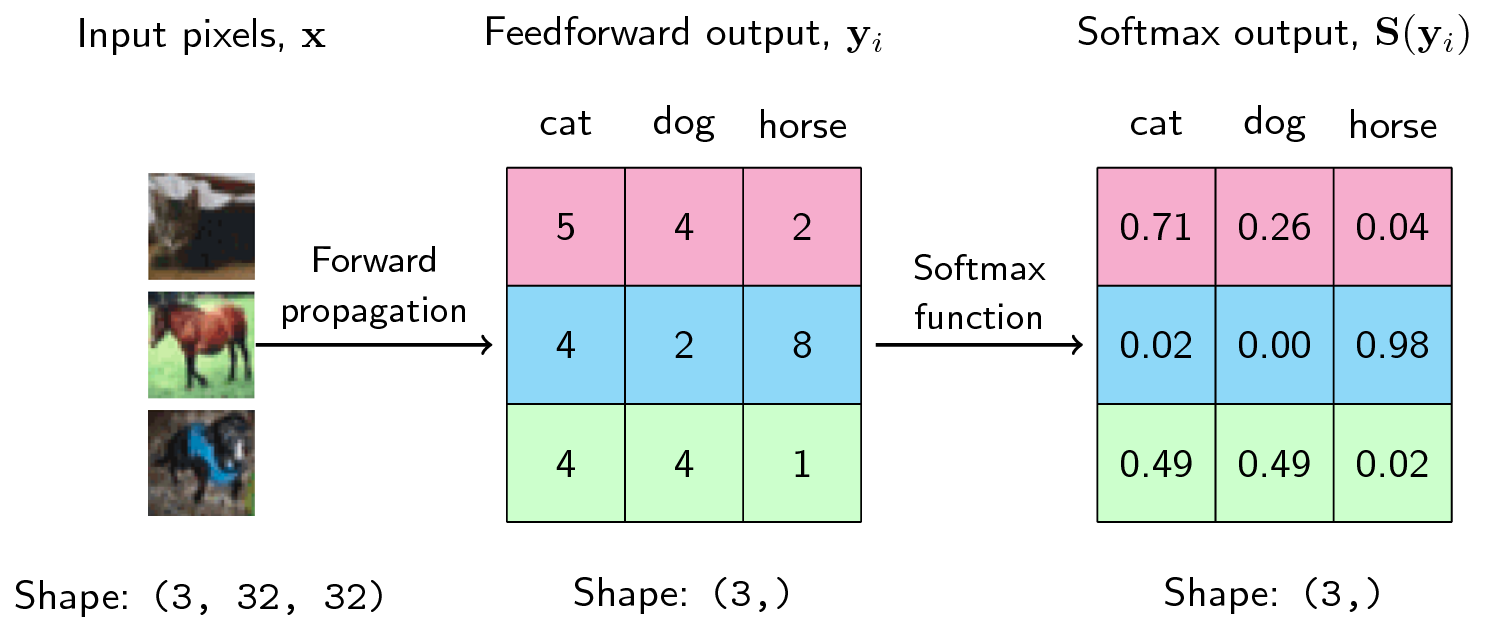
\includegraphics[width=.7\textwidth]{figures/chap3/ml/softmax}
    \caption{Intuitive example of the softmax function. In left the input data for each class. In right the softmax output aggregating to 1.}
    \label{c3:softmax}
\end{figure}

\subsection{Loss/Cost function}

When the forward pass is completed the network output $\hat{y}$ should be compared with the real values (groundtruth) in order to measure the discrepancy. Based on the definition from Section~\ref{c3:ml}, measuring the error between the prediction and the groundtruth, informs us of how good or bad the network performs during the training process. To measure the error, a \textit{loss} function will be utilised.

For \textit{linear regression} type problems, where the predicted $\hat{y}$ and groundtruth $y$ are continuous variables, we use the Mean Squared Error (MSE).

\begin{ceqn}
\label{c3:mse_eq}
\begin{align}
  \text{MSE}(y, \hat{y}) = \sum_{i=1}^{N} (y_i, \hat{y_i})^2
\end{align}
\end{ceqn}

MSE loss function is minimized when the predicted value $\hat{y}$ is as close enough to the groundtruth $y$.

For \textit{classification} problems the groundtruth values $y$ are encoded to vectors in length of the number of classes. This encoding is known as \textit{one-hot} encoding. More specifically each label $y_i$ is a binary vector, where its digit represent a class \textit{C}. A position with 1 in the vector, denotes the relative class. An example of an one-hot encoded vector is shown bellow.

The available class labels representing three digits are \textit{one, two} and \textit{three}.
\begin{ceqn}
\label{c3:one_hot_example}
\begin{align*}
  \text{digit} \rightarrow \text{(one two three)}
\end{align*}
\end{ceqn}

Each digit's label is one-hoe encoded in a binary vector.

\begin{ceqn}
\begin{align*}
        \begin{pmatrix} one \\ two \\ three \end{pmatrix} & \rightarrow \begin{pmatrix} 0 & 0 & 1 \\ 0 & 1 & 0 \\ 1 & 0 & 0 \end{pmatrix}
\end{align*}  
\end{ceqn}
\\

The loss function that is used in classification problems is called \textit{categorical cross-entropy}.

\begin{ceqn}
\begin{align}
  \text{J}(y, \hat{y}) = -\sum_{i=1}^{N} y_i \cdot \log \hat{y_i}
\end{align}  
\end{ceqn}
\\

The minimization of the loss function equals to the maximization of the posterior prediction that a network gives for a certain input $x_i$ to correspond to a class label $y_i$. In other words, we are looking for the \textit{Maximum Likelihood Estimation} (MLE).

\subsection{Learning process}

Now that we have defined most of the essential components of a neural network, we are going to discuss about the learning process.
Learning process is as iterative method that is carried over in \textit{epochs} and stops when a criteria is met. Our true objective is to find those network's parameters weights $W$ and biases $b$ that minimize the error of the cost function as intuitively presented in Figure~\ref{c3:wnb}.

\begin{figure}[h!]
    \centering  
    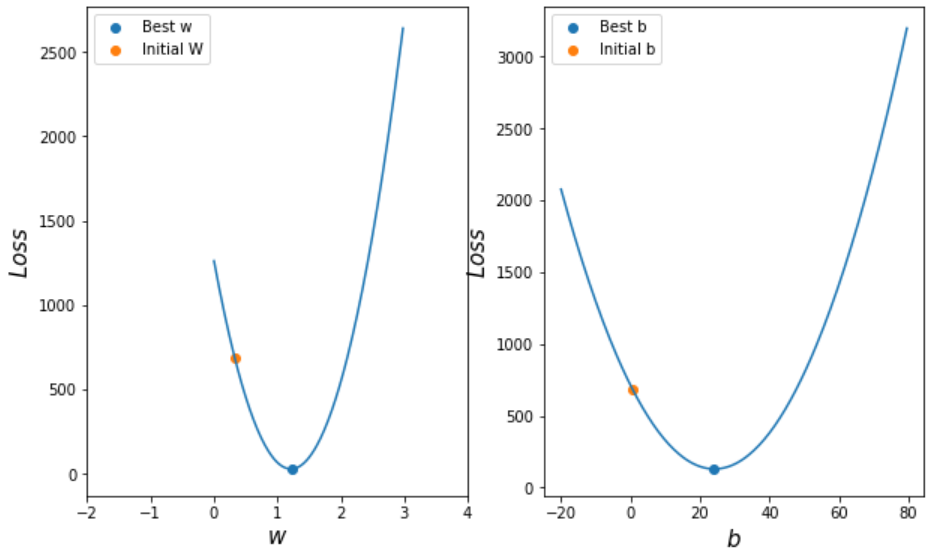
\includegraphics[width=.8\textwidth]{figures/chap3/ml/wnb}
    \caption{Initial and best weights and biases values hitting a local minima}
    \label{c3:wnb}
\end{figure}


During the forward pass, a sample is passed through the network of neurons until the final layer which outputs a posterior probability and the loss function calculates the error between the prediction and the groundtruth. Given the discrepancy, we need to inform the network about the error and adapt its parameters and start over. The problem is considered an optimization process and can be solved utilising a method called \textit{gradient descent}. By computing the gradients of the loss function with respect to each of the parameters $W$ and $b$ we are calculating the slope of the function to be approximated, at the current positition. The slope shows the direction that will follow in order to reduce to cost function's value.
For example, we calculate the weight's matrix $W_i$ as follows:

\begin{ceqn}
\begin{align}
    \nabla_{W_i}\text{J}(y, \hat{y}) = \frac{\partial\text{J}(y, \hat{y})}{\partial W_i}
\end{align}  
\end{ceqn}

and the updated value for the next epoch is given by:

\begin{ceqn}
\begin{align}
  W_{i}^{e+1} \leftarrow W_{i}^{e} - \lambda \cdot \frac{\partial\text{J}(y, \hat{y})}{\partial W_{i}^{e}}
\end{align}  
\end{ceqn}

where $\lambda$ is the \textit{learning rate} hyperparameter and dictates the magnitude of the update. Smaller values will require more steps for a network to converge, larger values might lose the minima and the network might never converge.
The above method can be consider a criterion to be met and the procedure is referred as \textit{training process} or \textit{fitting} while each learning cycle is referred as an \textit{epoch}.

For network architectures with multiple layers, a chain rule is applied to calculate the gradients of the layers next.

\begin{ceqn}
\begin{align}
    \frac{\partial\text{J}(y, \hat{y})}{\partial W_{i}} = \frac{\partial\text{J}(y, \hat{y})}{\partial z_{L-1}} \cdot \frac{\partial z_{L-1}}{\partial z_{L-2}} \cdot  \ldots  \cdot \frac{\partial z_{i}}{\partial W_{i}}
\end{align}  
\end{ceqn}
\\
For computational reasons, layers are updated backwards from the latter to the former, this operation is referred as \textit{backpropagation}.

\subsection{Optimization}

Overall, the main steps of machine learning are to build a model hypothesis (\textbf{M}), define the objective function (\textbf{J}) and solve the maximum or minimum of the objective function to determine the parameters (\textbf{w,b}) of the model.
The first two are the modelling problems of machine learning and the latter is to train the model by an optimization algorithm (optimizer).

An optimizer in deep neural networks is involved in many contexts. The simplest form used is the \textit{gradient descent} of the previous section.
An optimizer in general focuses on to find the parameters \textbf{$\theta$} of a neural network that significantly reduce a cost function $J(\theta)$~\cite{Goodfellow2016}.

\textit{Gradient descent} follows a global optimal solution, where all training samples \textit{N} are involved towards the calculation of the cost and when the objective function is convex like, similar to Figure~\ref{c3:wnb}.
Because this problem is very important and can become very expensive in applications with hundreds or millions trainable parameters that a specialized set of optimization techniques have been developed for solving it.

A variant of the above technique called \textit{Stochastic Gradient Descent} (SGD) uses a random sample \textit{i} rather than all samples, to update the gradient per iteration. That particular sampled is called \textbf{batch} while the cardinality of samples included in batch define the \textbf{batch size}.
\begin{ceqn}
\begin{align}
 \theta^{i+1} = \theta^i - \lambda \cdot \partial_{\theta^i} J(y_b,\hat{y_b}), b \subset N
\end{align}
\label{c3:eq_sgd}
\end{ceqn}
For every batch \textit{b} on iteration \textit{i}, SGD calculates the cost and updates model parameters in Equation~\ref{c3:eq_sgd}. After N/b iterations, when all samples \textit{N} have passed ones from SGD an \textit{epoch} is completed.

The main advantage of this method is that it does not require to load the entire set in memory, but only a batch. This technique enable training feasible for larger volume of data sets and despite the more iterations needed, this method is faster as since less computational time is less. It is also observed that SGD has regularization effects in training, as it mitigates overfitting~\cite{sun2019survey}.

Other successful variants of SGD, extend the equation with \textit{momentum}, an idea that derived from the mechanics of physics and preserves the influence of the previous update direction on the next iteration to a certain degree developing a mechanism to overcome local minima.
\begin{ceqn}
\begin{align}
 u^i = \lambda \cdot \partial_{\theta^i} J(y_b,\hat{y_b}) + \gamma u^{i-1}
\end{align}
\label{c3:eq_sgd_momentum}
\end{ceqn}
Momentum term is the $\gamma u^{i-1}$. If the update of the previous iteration  $u^{i-1}$ is high, then it will increase also the current iteration and thus the update is more increased. 
Other modern optimizers~\cite{kingma2014adam},~\cite{zeiler2012adadelta},~\cite{ duchi2011adaptive},~\cite{dozat2016incorporating}, utilise the above concept to optimize the momentum calculation and contribute to smoother gradient descent progression and ensure that training will converge.

\subsection{Bias and Variance}

Bias and variance are two types of errors that a classifier is subjected to make.
\textit{Bias} occurs from the false estimations during training. In neural networks, bias may arise when the network complexity is very simple, namely it does not have the capacity to learn more complex representation of the input \textit{X} related the label \textit{y}. For example, if the task is complex and a low capacity or complexity network is used, high bias is expected to occur. High bias is also referred as underfitting. An example of classifier with high bias is visualized in Figure~\ref{c3:fig_bias}.

\begin{figure}[h!]
    \centering  
    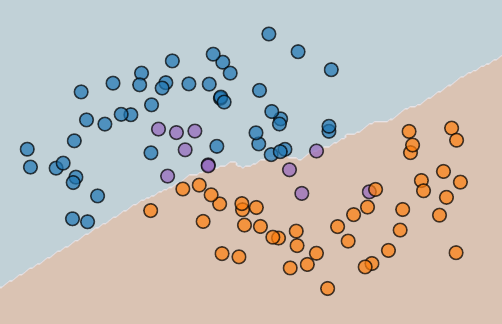
\includegraphics[width=.7\textwidth]{figures/chap3/ml/bias}
    \caption{Example of a classifier with high bias. Circles are the samples \textit{X}. Blue and orange are the corresponded class that a sample is assigned, while in purple are the false predictions. A linear classifier has not the ability to learn the non-linear complexity of that particular data set.}
    \label{c3:fig_bias}
\end{figure}

\textit{Variance} is a concept related to bias which derives from the classifier's sensitivity in minor input changes. In practice, means that the classifier can capture random variation in input such noise or from random behavior in the learning algorithm itself, such random initial weights~\cite{dietterich1995machine}.  An example of classifier with high variance is visualized in Figure~\ref{c3:fig_variance}.

\begin{figure}[h!]
    \centering  
    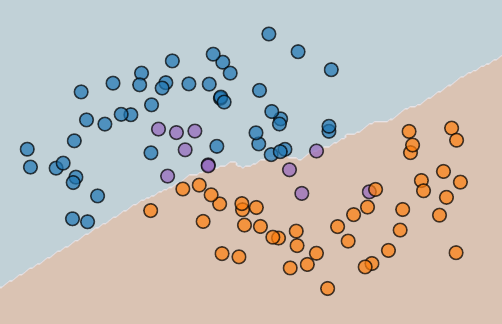
\includegraphics[width=.7\textwidth]{figures/chap3/ml/bias}
    \caption{Example of a classifier with high variance. The decision line is overfitted on the samples as the classifier has learned perfectly the data set. That will cause issues in task generalisation.}
    \label{c3:fig_variance}
\end{figure}

\subsection{Objective performance evaluation}

To prevent classifier from overfitting and ensure the proper network generalisation, we ``hide'' completely a portion of the data from the classifier during training and use it only for evaluation. In this way, we divide the data set \textit{X}, in two subsets: \textit{train set} $X_{train}$ and \textit{test set} $X_{test}$ as in Figure~\ref{c3:fig_train_test}.

\begin{figure}[h!]
    \centering  
    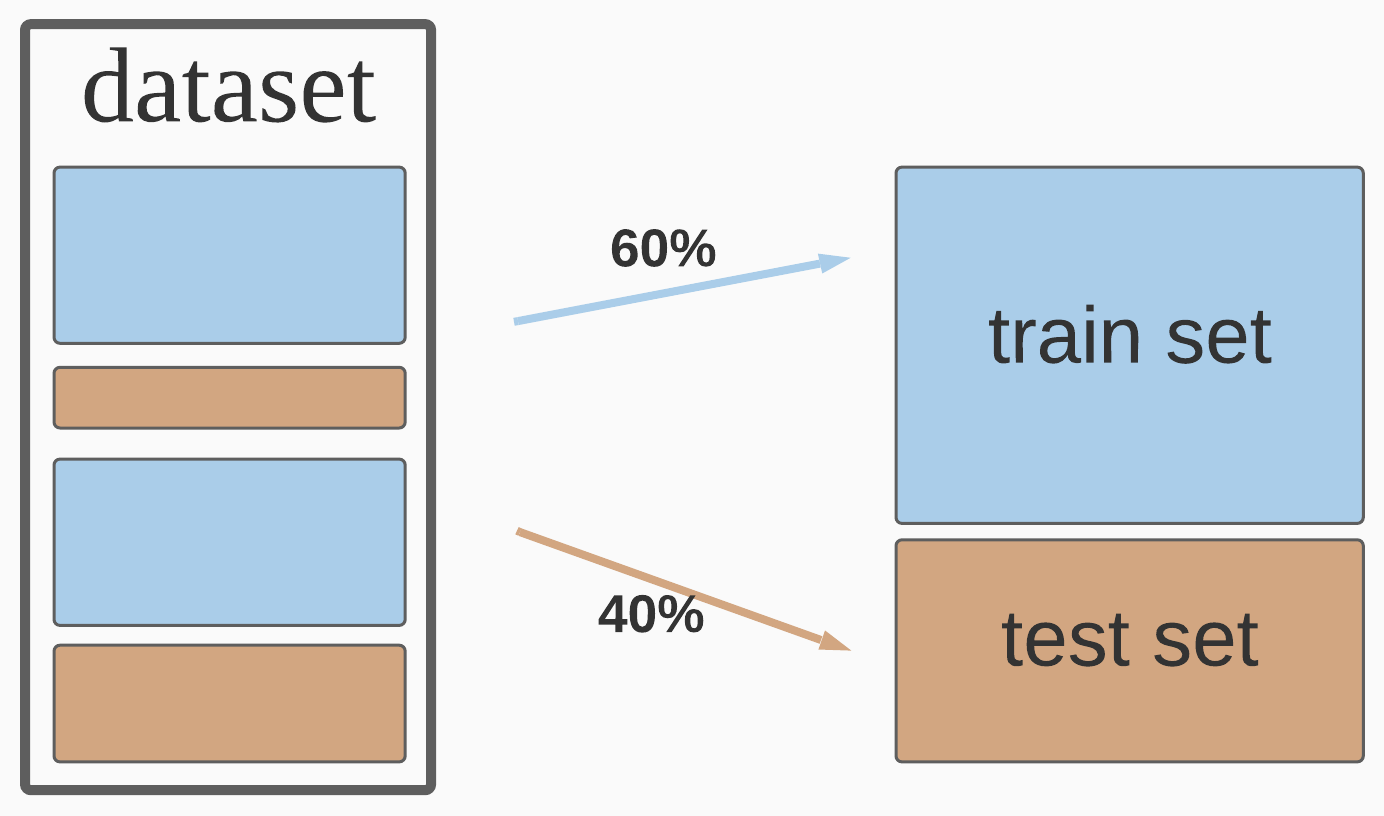
\includegraphics[width=.6\textwidth]{figures/chap3/ml/train_test}
    \caption{Data set split in 2 subsets: a train set and a test set by 60/40 ratio.}
    \label{c3:fig_train_test}
\end{figure}

In cases with extended experiments, the risk to overfit the network's hyperparameters to a certain test set is increased. To prevent the selection of hyperparameters that perform well only on the selected test set, we create a third subset, the \textit{validation set} $X_{val}$. 
A common practice to acquire a validation set is to split the existing training set or in case where access to large sets of data in not the case validation can have the same ration as the test set.
In practice, the network is trained as usual and the validation set is used in order to tune hyperparameters and set the model's weights. 
The final model is evaluated on the test set (Figure~\ref{c3:fig_train_val_test}).

\begin{figure}[h!]
    \centering  
    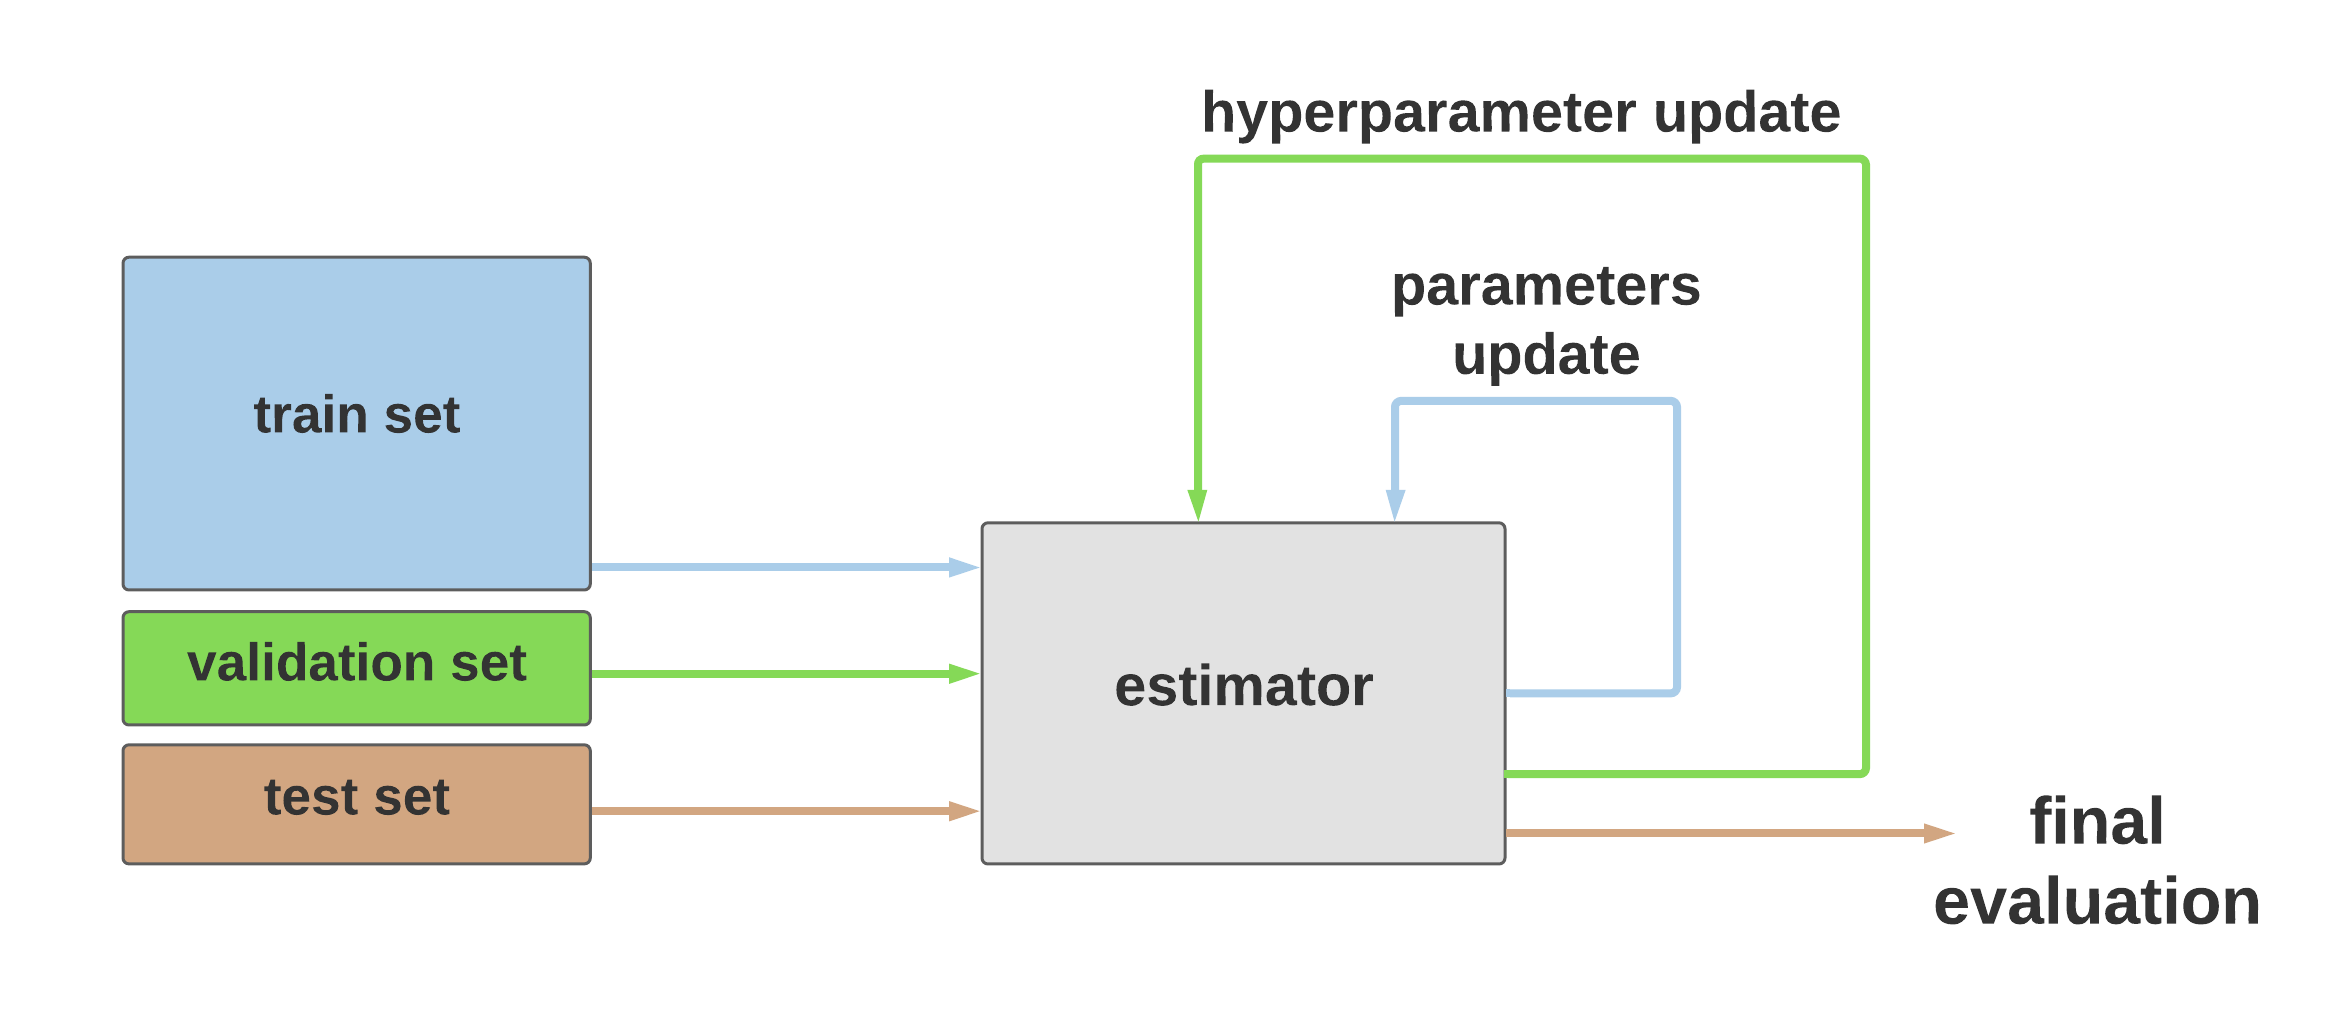
\includegraphics[width=.8\textwidth]{figures/chap3/ml/train_valid_test}
    \caption{Training process of an estimator. Train set is used to update model's parameters(weight and biases). Validation set is used to tune model's optimal hyperparameters. Test set is used for the objective performance evaluation of the classifier.}
    \label{c3:fig_train_val_test}
\end{figure}


\section{Regularization}

Training a deep neural network is considered an art rather than a typical procedure. The choice of hyperparameter is not limited in the number of layers, convolution filter size etc.  but is expanded to the subtle selection of other hyperparameters. Some of them are weight initialization techniques, learning rate decay, early stopping, dropout and batch normalization layers.

In this section we will discuss about dropout and batch normalization since the rest of techniques are briefly presented in Section~\ref{c5:section_passive_learning}.

\textbf{Dropout}~\cite{srivastava2014dropout} is one of the oldest regularization techniques in deep learning, Figure~\ref{c3:fig_dropout}. At each training iteration, it drops random neurons from the network with a probability p (typically 25\% to 50\%). In practice, neuron outputs are set to 0. The net result is that these neurons will not participate in the loss computation this time around and they will not get weight updates. Different neurons will be dropped at each training iteration.

\begin{figure}[h!]
    \centering  
    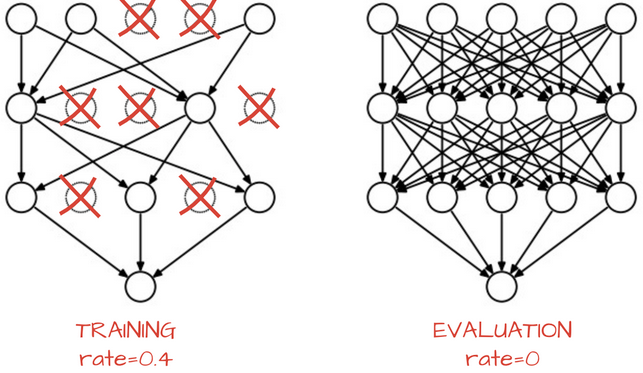
\includegraphics[width=.7\textwidth]{figures/chap3/ml/dropout}
    \caption{Dropout demonstration during training with 40\% neuron drop. In evalution(inference) all the neuron are used.}
    \label{c3:fig_dropout}
\end{figure}

A more complex technique called \textbf{batch normalization} tries to address a problem, known as \textit{internal covariate shift}~\cite{ioffe2015batch}, which relates to how neuron outputs are distributed relatively to the neuron's activation function by the time. 
At the beginning, network parameters are randomly initialized while during training these parameters are varying. The variations in the distribution of neuron's activations has a property to ``confuse'' the next layer and so forth to destabilize the training.\

In the bottomline, \textit{batch normalization} aims to stabilize the training process by minimizing exploding gradient issues, helps the network to converge and usually allows to decrease the dropout rate, or even acts as a substantial to regularize overfitting.

\section{Convolutional Neural Networks}

Deep neural networks are hierarchical learning systems, in which high-level features are obtained by composing the low-level ones. In images, local combined features of edges form motifs, motifs assemble into parts and parts create objects.
Convolutional neural networks (CNN) are inspired by neuroscience and more specifically the overall architectures mimic the human visual cortex, as we showed in Section~\ref{c2:sec_iaqa}.
Marr~\cite{marr1982vision} claimed that the attributes carrying the valuable information in an image, may emerge at any of a range of scales in the real world.
He formulated a physical assumption on hierarchical organizations of the visual world that in simple terms supports that the human representation mechanism must work under a number of different scales in order to capture changes in \textit{depth} and \textit{surface orientation}.

The above statement is the core function in the design of a CNN. Convolutional networks are designed to process data that come in its raw form, for example a colour image is composed of three 2D arrays containing pixel intensities in RGB colour space. That itself, is a major breakthrough in the domain of pattern recognition, as the use of handcrafted features becames obsolete.

The key ideas behind a CNN can be considered the following:

\begin{itemize}
 \item Automatic feature engineering
 \item Parameter sharing
 \item Local connections
 \item Pooling
 \item Non-linearity
 \item Used in many layers
\end{itemize}

The architecture of a typical CNN in illustrated in Figure~\ref{c3:fig_cnn} and is structured as a series of stages.

The first stages are composed of two types of layers: convolution and pooling layers.

\begin{figure}[h!]
    \centering  
    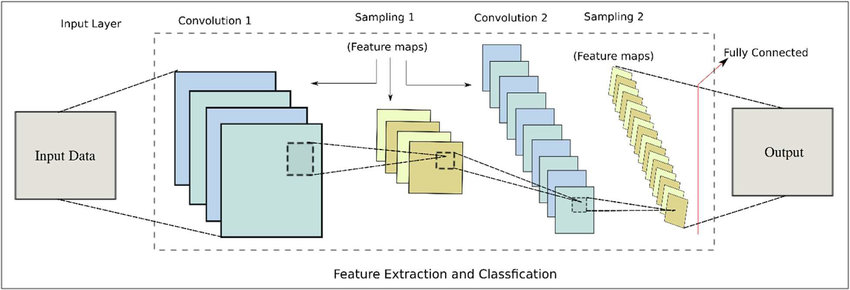
\includegraphics[width=.7\textwidth]{figures/chap3/cnn/cnn_sample}
    \caption{A typical convolution neural network architecture.}
    \label{c3:fig_cnn}
\end{figure}

In a convolution layer, the units are organized in features maps, Figure~\ref{c3:fig_feature_map}, within each unit is connected to local patches in the feature maps of the previous layer through a set of weights(parameter sharing), using a pool of filters. 

\begin{figure}[h!]
    \centering  
    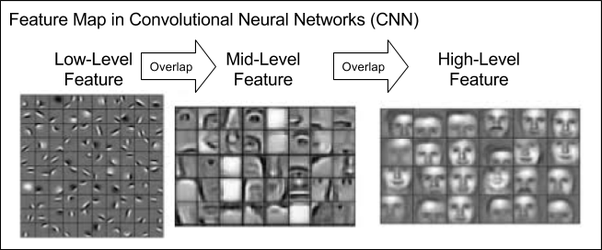
\includegraphics[width=.7\textwidth]{figures/chap3/cnn/feature_map}
    \caption{A hierarchical feature map from low to high level features.}
    \label{c3:fig_feature_map}
\end{figure}

The result of this local weighted sum is then passed through a non-linear function such a ReLU. All units in a feature map share the same filter pool while different feature maps in a layer use different filter pools.

The reason for this technique is twofold.
First, in a image, local groups of values are often highly correlated and form distinctive local motifs that are easily detected.
Second, the local features of images are invariant to translation. More specifically, if a motif may appear in any region of an image, the same pattern can be detected in any region, since units at different locations share the same weights.

However, the role of a convolutional layer is to detect local organizations of features from the previous layers, the role of pooling layer is to merge the semantically similar features into one. A typical pooling layer computes the max or average value of a selected set of output neurons from the convolutional layers and use these as inputs to higher layers.
Because of the relative posititions of the features forming a motif can vary, effective detection can be achieved by downsampling the patch region of each feature, giving the property of invariance to shifts and distortions of the inputs.

After the last concolutional layer, the data is in the form of a ``cube''. In order to pass to the next stage of a CNN, a densely connected layer, there are two ways.

The first one is to flatten the data into a vector and then pass it to the dense layer with a softmax activation.
The second and more cost efficient, is to average all the values and feed these through a softmax activation function. Figure~\ref{c3:fig_flatten_global} illustrates the two methods.

\begin{figure}[h!]
    \centering  
    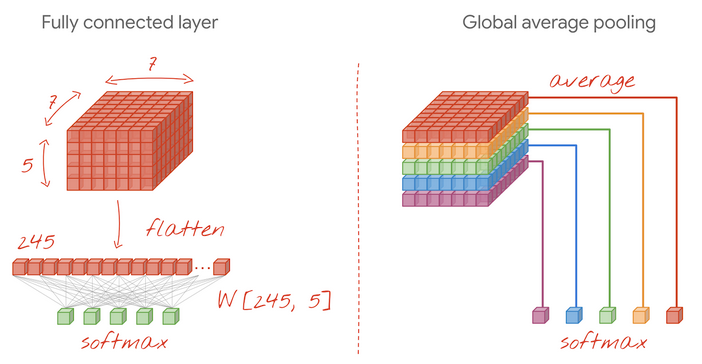
\includegraphics[width=.7\textwidth]{figures/chap3/cnn/flatten_global}
    \caption{Two methods to pass the input of the last convolutional layer to a densely connected layer.}
    \label{c3:fig_flatten_global}
\end{figure}


With these constraints, the model can be quite compact in terms of number of actual parameters. A CNN architecture achieves a substantial reduction in the number of connections concerning to a densely connected network via parameter/weight sharing and pooling layer.

Summing up, a convolutional neural network, is primarly comprised of two levels. The feature extraction level, that is constructed from convolutional and pooling layers, trained to extract better and more robust features. The layer properties allow the use of stacking multiple layers thus forming a deep network structure.
The second level, contain fully connected layers. This layers aim to learn the associations between high-level features of the last convolutional layer with the labels of the input in order to perform classification.

\subsection{Convolution and receptive fields}

In convolutional neural network the key operation is basic linera algebra operation where an a filter or kernel with a set of weights, slides on a input vector. In each slide, an element-wise multiplication between the input and the kernel in performed producing a dot product which is summed, resulting in a single value. Applying a filter to an image will result in a feature map that will have the characteristic of the filter element structure. The operation is visualised in Figure~\ref{c3:fig_convolution}(a). Different type of filters will results in a different feature map(vertical lines, horizontal lines).

By stacking multiple convolutional layers allows a hierarchical decomposition of the input, from low-level features expressed in lines or edges, to high-level features such objects, faces etc.

Pooling is a operation, without dot product level multiplications. Pooling layers does not have weight parameters and perform a simple pooling operation such meam, averaging or max pooling as illustrated in Figure~\ref{c3:fig_convolution}(b).


\begin{figure}[h!]
    \centering  
    \subfigure[]{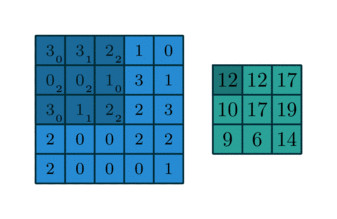
\includegraphics[width=.4\textwidth]{figures/chap3/cnn/conv}}
    \subfigure[]{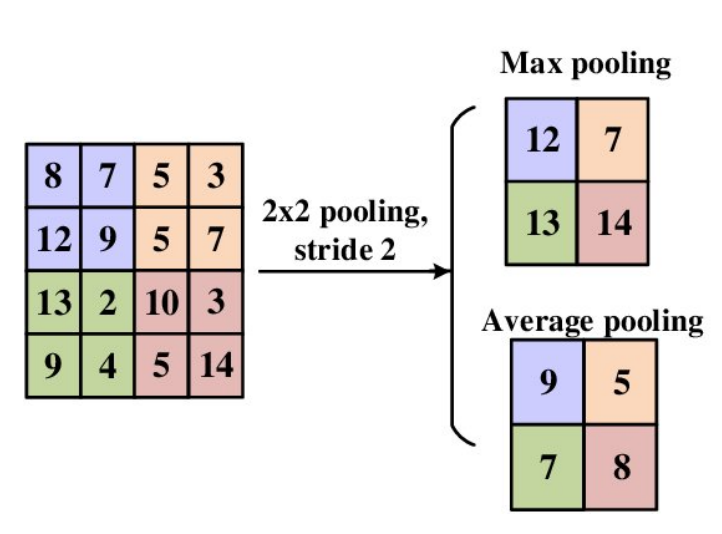
\includegraphics[width=.4\textwidth]{figures/chap3/cnn/pooling}}
    \caption{(a) The operation of convolution between an input(blue) and a kernel(dark-blue) with weights. The out of a single slide is a single number(dark-green). The whole operation produce a new feature map(green). (b) Pooling operation in max and average types of pooling.}
    \label{c3:fig_convolution}
\end{figure}

The notion of a \textit{receptive field} in a deep convolutional architecture is inspired from the human visual system, (Figure~\ref{c3:fig_receptive_field}-a).

In deep learning, the receptive filed is defined as the size of the region in the input that produces the feature~\cite{araujo2019computing}. Receptive field refers only to the feature extraction part of the network, because a convolution unit is connected or depends to only a specific region of the input.
Intuitively, the network's receptive field is the region of an input - not only the input of the network, but any input, can be the output of any network layer - with a relative unit that we consider it as output receiver of the input. For example a simple convolutional operation between a kernel and an input is considered a receptive field. Also the final convolutional layer in respect of the first input layer characterises the total network's receptive field size, (Figure~\ref{c3:fig_receptive_field}-b).

\begin{figure}[h!]
    \centering  
    \subfigure[]{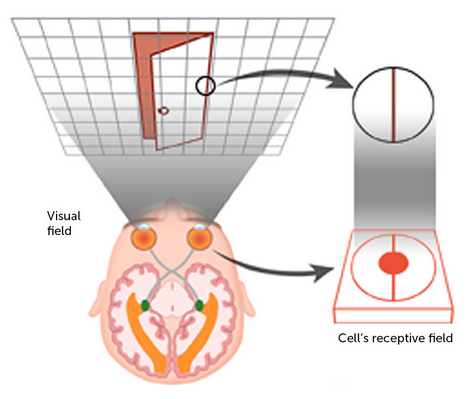
\includegraphics[width=.4\textwidth]{figures/chap3/cnn/human_receptive_field}}
    \subfigure[]{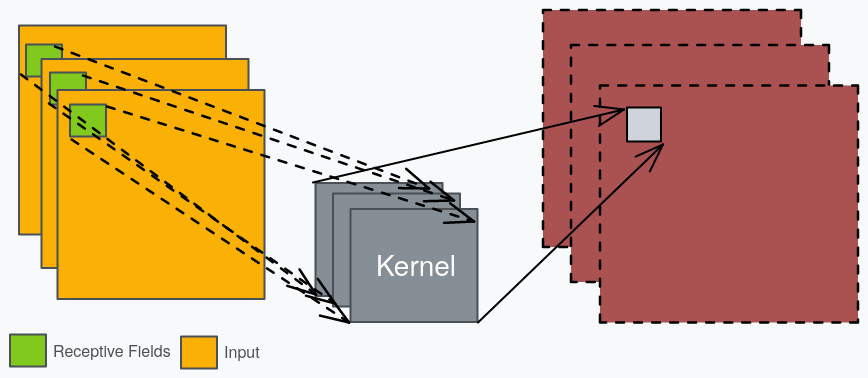
\includegraphics[width=.4\textwidth]{figures/chap3/cnn/receptive_fields}}
    \caption{(a)Human receptive field, (b) Receptive field with convolution operation.}
    \label{c3:fig_receptive_field}
\end{figure}

\section{Deep Learning Architectures}
\label{c3:deep_arch}

In order to increase the receptive field in a convolutional network, there is a variety of ways to achieve it. It can be done by adding more convolutional layers(make the network deeper, add pooling layers, increase convolution striding, use sequential dilated convolutions or add skip connections.
The latter has also regularization properties, because an the network becomes deeper the risk of vanishing gradient problem to appear is higher.

By using a skip connection, we provide an alternative path for the gradient(with backpropagation). At its name suggests, skip connectios, skip some layer in the network and feeds the output of one layer as the input to the next layers~\cite{adaloglou2020skip}.

There are two ways to apply skip connection, with \textbf{addition} and \textbf{concatenation}. In this thesis, we have applied the famous DenseNet~\cite{huang2017densely} architecture which utilises concatenations as skip connections (Figure~\ref{c3:densenet_arch_origin}).

\textit{DenseNet} model starts with a convolutional-pooling block and continues with a series of ``Dense blocks-Transition layer''. Finally it closes with a \textit{Global Average pool} and a \textit{Fully-connected} block.

In every ``Dense block'' the input tensor passes through a series of convolutional operations with fixed number of filters \textit{k} and the result of each one is then concatenated to the original tensor.

Thus the number of feature maps of the input tensor follows an arithmetic growth at every internal stage of the Dense block by \textit{k} tensors per stage.
In order for the size of the tensor to remain manageable the model makes use of the \textit{Transition layers} where the number of feature maps of the input tensor is reduced to half. Also the spatial dimensions of the input tensor are halved by an \textit{Average Pool layer}.

At each \textit{Dense block}, there is a repetition of: (a) $1\times1$ conv with $4\cdot k$ filter, (b) $3\times3$ conv with $k$ filters. Every \textit{Dense block} is constructed by Batch Normalization-ReLU-Convolution sets. The aforementioned modules of DenseNet model are shown in Figure~\ref{c3:densenet_arch_modules}

\begin{figure}[h!]
    \centering  
    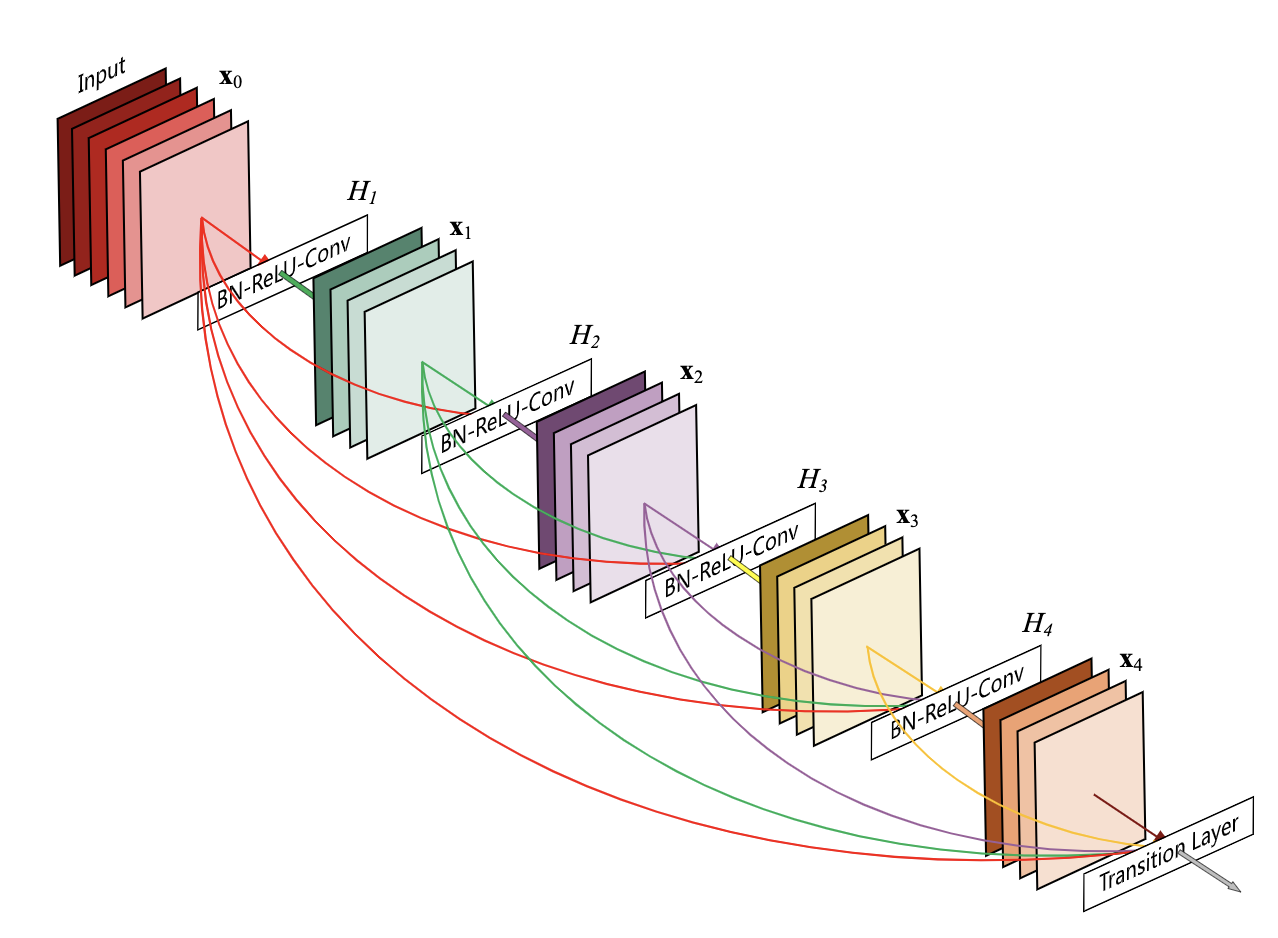
\includegraphics[width=.5\textwidth]{figures/chap3/cnn/architectures/densenet_arch_origin}
    \caption{DenseNet architecture from the original paper~\cite{huang2017densely}}
    \label{c3:densenet_arch_origin}
\end{figure}

\begin{figure}[h!]
    \centering  
    \subfigure[]{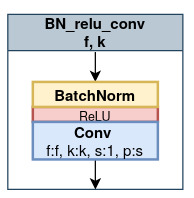
\includegraphics[width=.2\textwidth]{figures/chap3/cnn/architectures/densenet_1}}
    \subfigure[]{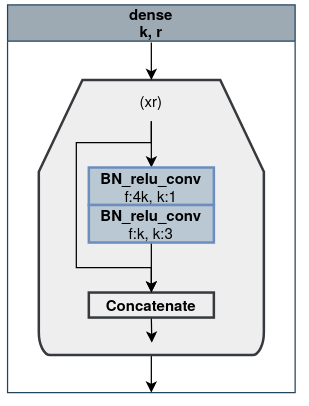
\includegraphics[width=.2\textwidth]{figures/chap3/cnn/architectures/densenet_2}}
    \subfigure[]{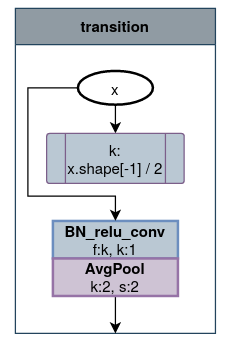
\includegraphics[width=.2\textwidth]{figures/chap3/cnn/architectures/densenet_3}}
    \subfigure[]{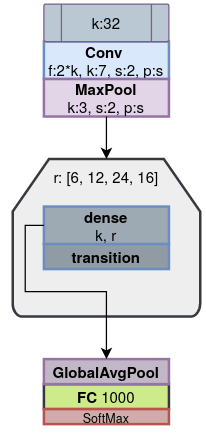
\includegraphics[width=.2\textwidth]{figures/chap3/cnn/architectures/densenet_4}}
    \caption{DenseNet model modules: (a) BN-ReLU-Conv compartment, (b) Dense block, (c) Transition layer, (c) all modules of the original DenseNet}
    \label{c3:densenet_arch_modules}
\end{figure}


More specifically we have implemented a lighter version of DenseNet architecture where more details are presented in Section~\ref{c5:section_passive_learning}, illustrated in Figure~\ref{c3:densenet_arch}.

\begin{figure}[h!]
    \centering  
    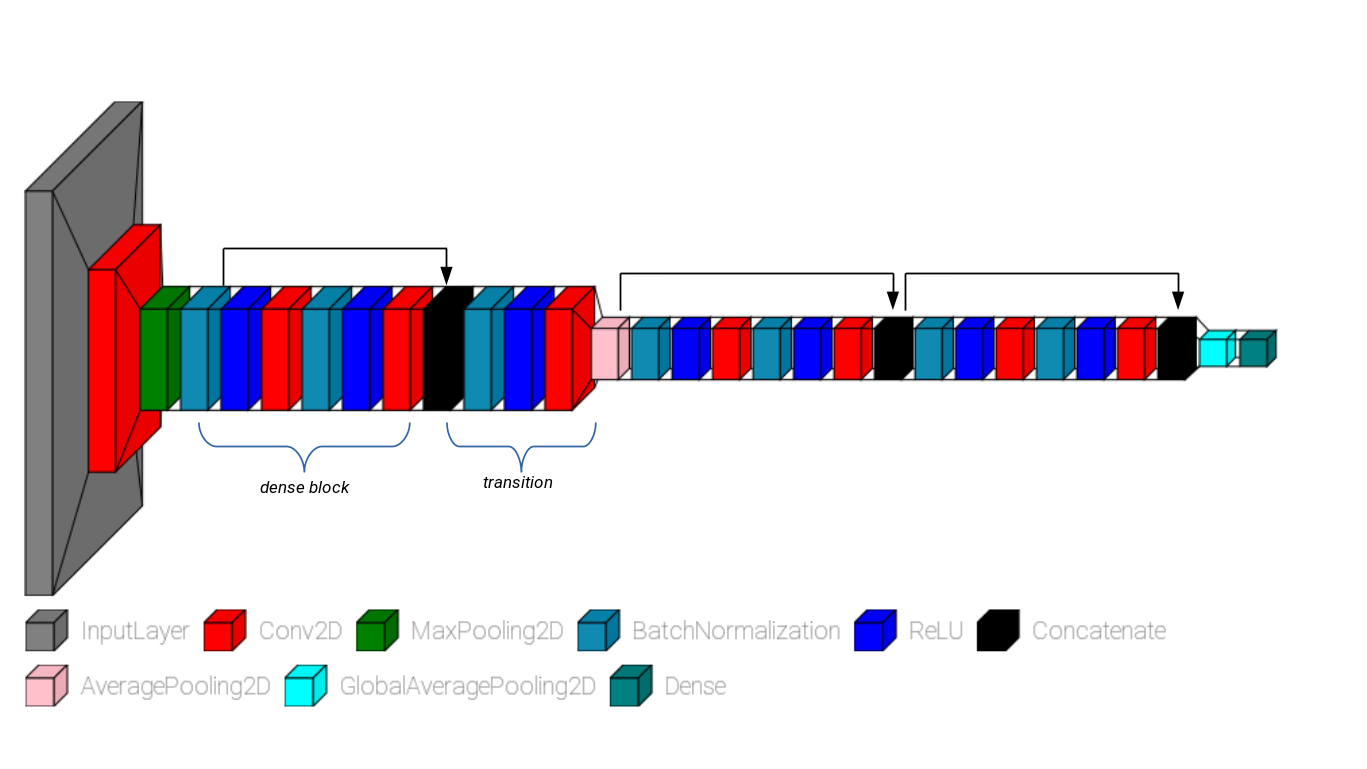
\includegraphics[width=.7\textwidth]{figures/chap3/cnn/architectures/densenet_arch}
    \caption{DenseNet architecture with 1 and 2 consecutive Dense Blocks}
    \label{c3:densenet_arch}
\end{figure}

Another famous architecture, the winner in ImageNet Challenge 2014, is the \textit{VGG16}~\cite{simonyan2014very}. It is a rather simple but very deep architecture of 16 layers. All hidden layers are equipped with ReLU non-linearity and max pooling is performed over a $2\times2$ window, with stride 2.
The network consists of 5 convolutional blocks and 3 fully connected layers. Each convolutional block consists of 2 or more convolutional layers and a max pool layer. 
In this thesis we utilised VGG16 with pretrained imagenet weights while we substitute the last decision layer with globar average pooling, a batch norm layer and a two-output softmax layer.
Figure~\ref{c3:vgg_arch} illustrates the network architecture.

\begin{figure}[h!]
    \centering  
    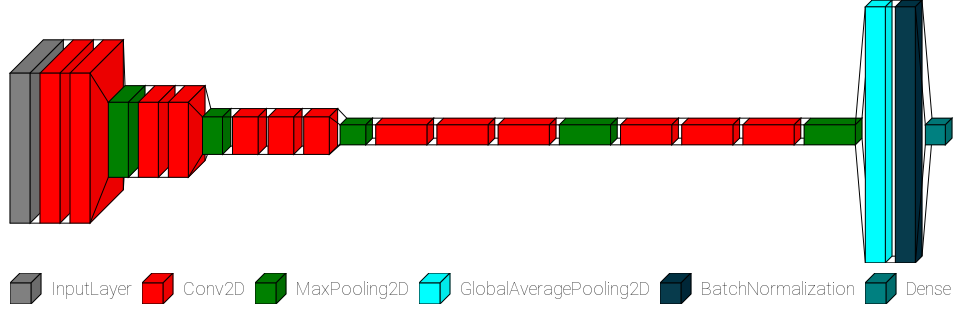
\includegraphics[width=.7\textwidth]{figures/chap3/cnn/architectures/vgg_arch}
    \caption{VGG16 architecture with Global Average Pooling 2D and Batch Normalization layers at the end}
    \label{c3:vgg_arch}
\end{figure}

Moreover, we have created a SimpleNet architecture, inspired from the aforementioned models. We have combined the notion of Dense blocks in DenseNet with the deep layer architecture of VGG16. The network consists of 3 convolutional block and 2 fully connected layers. Each convolutional block consists of 2 or more convolutional layers and a max pool layer. The first layer is consisted of one Dense block, while the rest of two Dense block. After the last convolutional layer a global average pooling layer forwards the input to a fully connected layer, passed to a Dropout, to a softmax decision output.
Figure~\ref{c3:simplenet_arch} depicts the network architecture.

\begin{figure}[h!]
    \centering  
    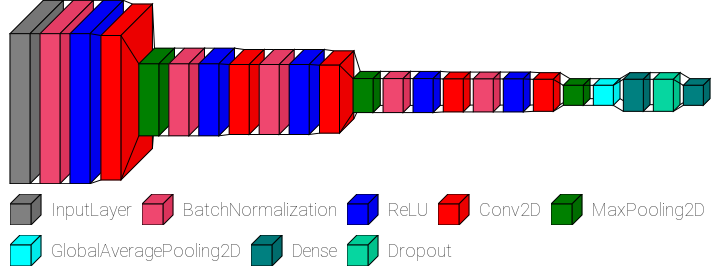
\includegraphics[width=.7\textwidth]{figures/chap3/cnn/architectures/simplenet_arch}
    \caption{A SimpleNet architecture}
    \label{c3:simplenet_arch}
\end{figure}

More details of the network can be found in Section~\ref{c5:section_passive_learning} and in Appendix.

%%%%%%%%%%%%%%%%%%%%%%%%%%%%%%%%%%%%%%%%%%%%%%

\section{Image Aesthetics with Deep Learning}
\label{c3:section_aesthetics_deep}
Image aesthetics quantification is a task that has gained tremendous growth with the use of deep learning techniques from 2014 and later. The research community has adopted the term Image Aesthetics Quality Assessment (IAQA)~\cite{yang2019comprehensive} to approach the problem, which can be divided in five different aesthetic tasks including aesthetic classification, regression, distribution aesthetic factors and description.

Deep learning, like to many other applications, offers and automatic and universal solution to extract features and consequently learn a feature extractor solely based on the input data. In contrast with traditional hand-made feature extractors that require substantial amount of engineering skills and domain expertise, a deep learning approach does not require to master complicated and demanding knowledge.

Major developments in the domain such as the dramatic improvement in the ImageNet classification benchmark from Krizhevsky et al~\cite{krizhevsky2012imagenet} using a DCNN, and the release of the \textit{Analysis of Visual Aesthetics}(AVA) data set in the same year from Murray et al~\cite{murray2012ava}, which contains over 250,000 photos from \textit{DPChallenge.com}, put IAQA again in the spotlight.

Summarizing the recent literature concerning aesthetic classification and regression related tasks in 2014, Lu et al~\cite{lu2014rapid}, proposed RAPID(RAting PIctorial aesthetics with Deep learning) system which adopts a double-column DCNN which combines heterogenous inputs from global and local view of an image to create a unified classifier using AVA dataset.

In 2016, Kong et al~\cite{kong2016photo} assembled a new aesthetics and attributes database (AADB) which contains aesthetics scores in form of star-rating and meaningful attributes mapped to each image given by multiple human annotators. In addition they have proposed a new CNN architecture that unifies aesthetics attributes and photo content for image aesthetic ratings upon a classification problem benchmarking their published data set versus AVA.
Their published data set were collected in co-operation with professional photographers and is closely related to image aesthetic judgements such content, object emphasis, light, colour harmony, vivid colour, shallow depth of field, motion blur, rule of thirds, balanced elements, repetition and symmetry.


Another approach that focus on preserving the image composition fed to a CNN, without damaging the input image by a geometric transformation is proposed by Mai~\cite{mai2016composition}, 2016. Multi-Net Adaptive Spatial Pooling ConvNet(MNA-net) is a compotition-preserving architecture which learns aesthetics features from images retaining their original aspect ratio without any transformation achieved by an adaptive spatial pooling layer on regular convolutional layers placed in network's input. It also allows multi-scale feature extraction achieved from multiple sub-networks with different adaptive spatial pooling sizes, also utilising AVA data set.


A work in 2017 from Malu et al~\cite{malu2017learning} similar to Kong's, attempts to interpret image quality attributes contributing to an overall aesthetic score. They propose a multi-task dcnn which simultaneously learn eight aesthetic attributes the same as above, composition balance, content, colour, depth of field, light, object emphasis, rule of thirds and vivid colours, along with the overall aesthetic score Figure~\ref{c3:aadb}. The have also developed a visualization of feature map activations based on the attributes above to highlight the key regions that correspond to the related feature attribute using the AADB database.

A recent study attempts to solve the same problem by training a dcnn to recognize if an image is appealing or not. Bhandari et al~\cite{bhandari2020image} incorporate a technique that extracts low-level features such colour properties and high level features in order to recognize prominent structures and entities in an image such, salient objects, rule of thirds, depth of field and other. They have created a diversely collected data set from Google, Flickr, Kaggle and at the same time utilize the GrabCut algorithm to efficiently extract the foreground object from a complex environment.

However, inspecting the data sets used in the aforementioned papers, the distinction between ``high'' and ``low'' quality images is more of a stylistic difference than anything else. Figure~\ref{c3:crap} shows a sample from AADB dataset and there is a profound evident of the content quality. Also, Figure~\ref{c3:ava_crap}, shows the image aesthetic classification from the RAPID system.
We would argue, that this style of photography is not by any means close to a known form of art. One can observe, datetime captions, poor sharpness, flat and overwhelming shots from compact cameras or even mobile devices.
Photography is a form of art that adopts the aspect of the visual world and extends it, in the undefined rules of a form that a photographer chooses to transform into a new medium of communication.

\begin{figure}[ht!]
    \centering  
    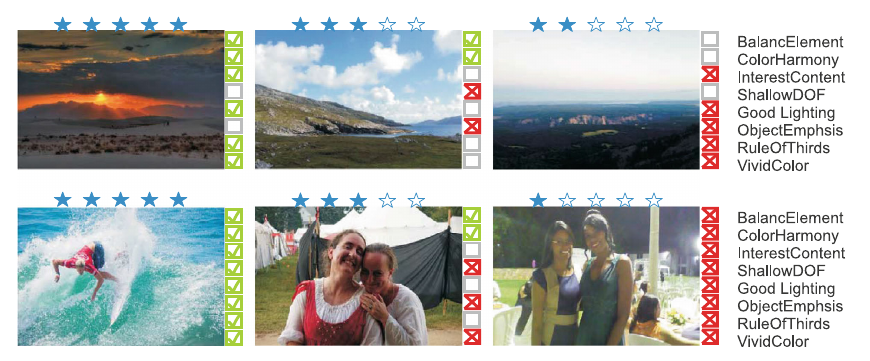
\includegraphics[width=.6\textwidth]{figures/chap2/aesthetics/aadb_dataset}
    \caption{Sample images in AADB dataset. Each photo is annotated with 8 aesthetic attributes in binary labels and aesthetic ratings.}
    \label{c3:aadb}
\end{figure}

\begin{figure}[ht!]
    \centering  
    \subfigure{{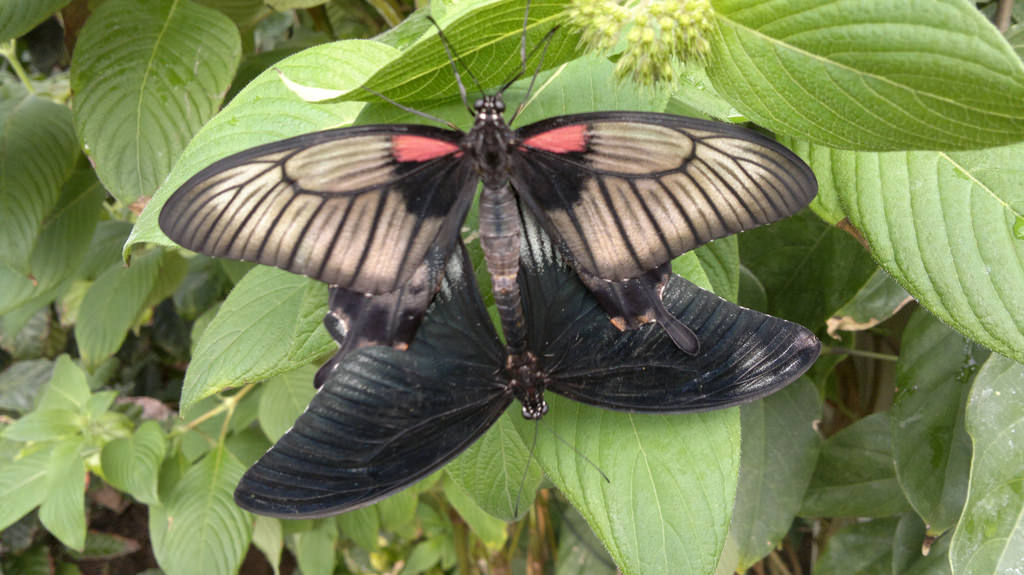
\includegraphics[width=.2\textwidth]{figures/chap3/crap/1}}}
    \subfigure{{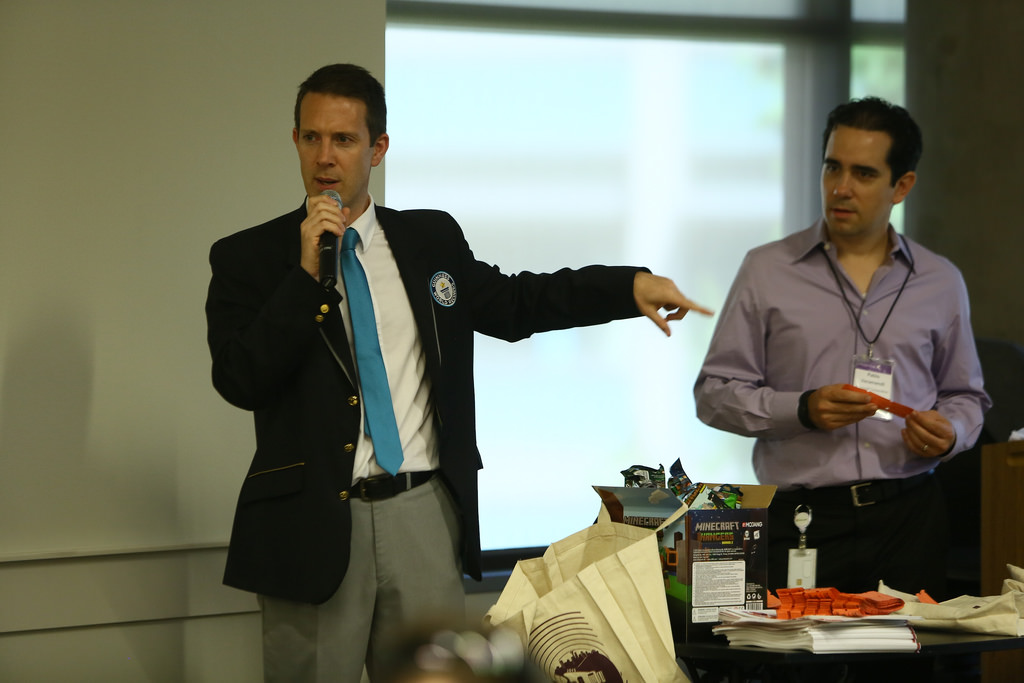
\includegraphics[width=.2\textwidth]{figures/chap3/crap/2}}}
    \subfigure{{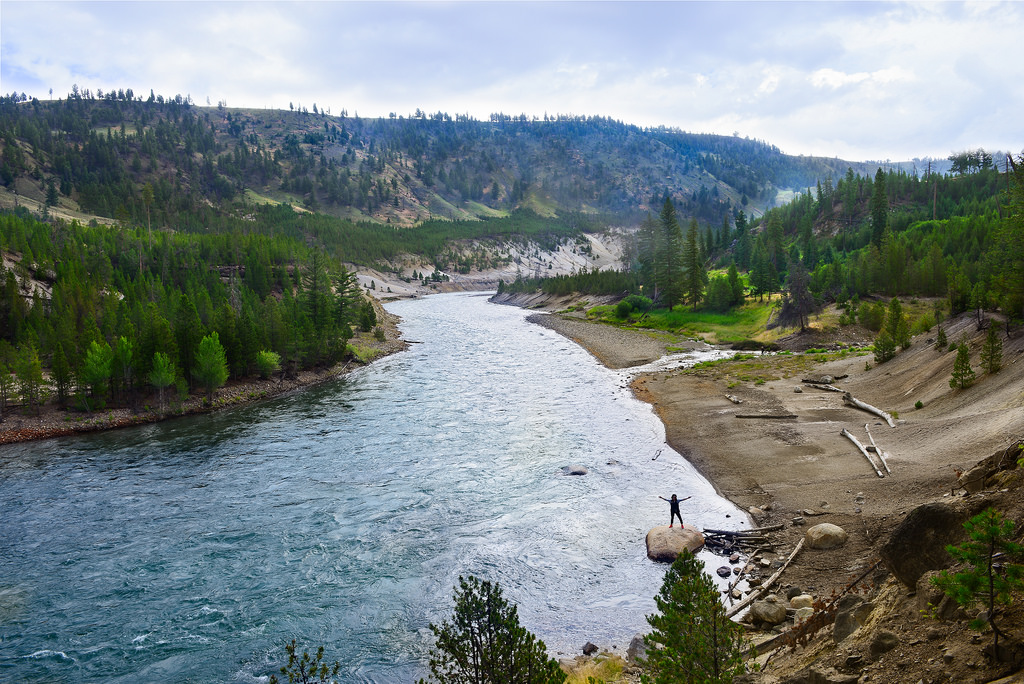
\includegraphics[width=.2\textwidth]{figures/chap3/crap/3}}}
    \subfigure{{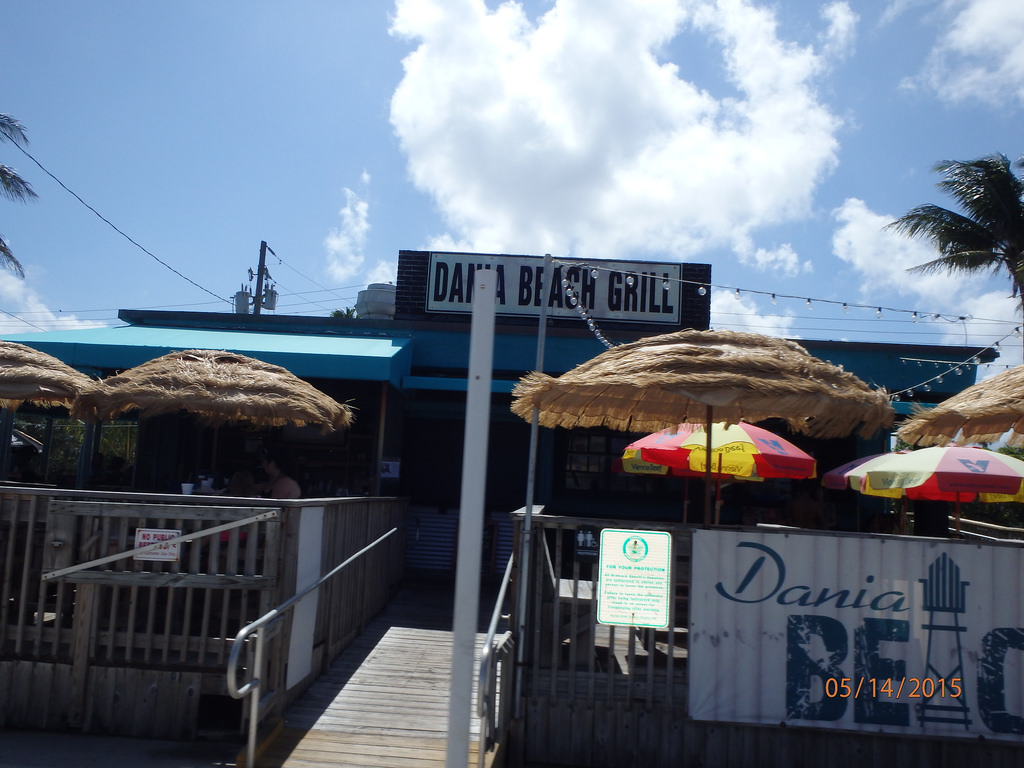
\includegraphics[width=.2\textwidth]{figures/chap3/crap/4}}}
    \subfigure{{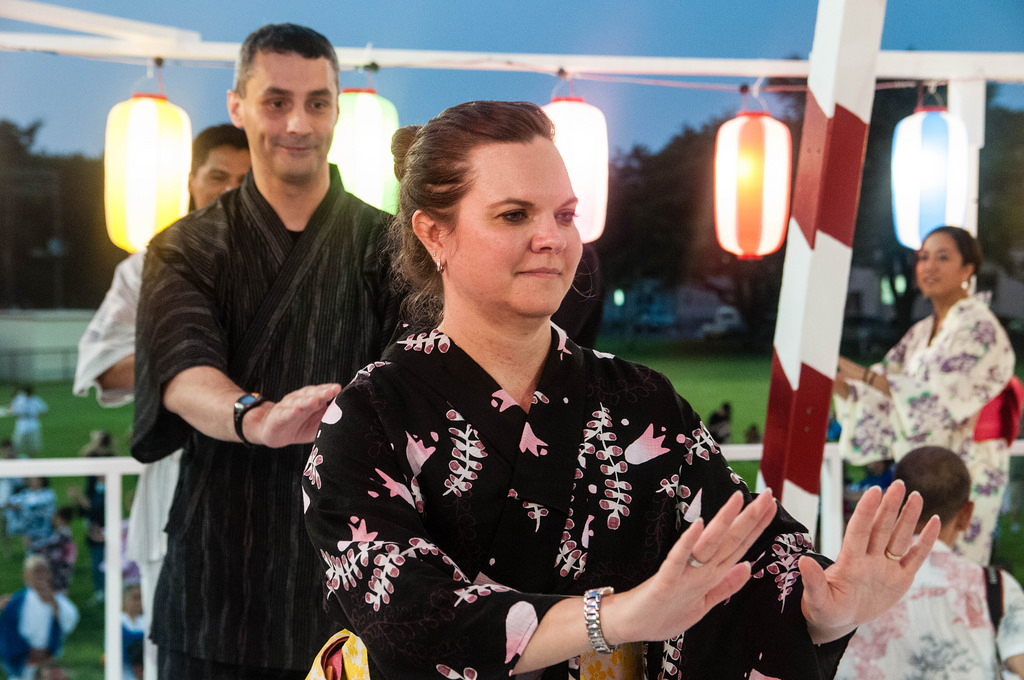
\includegraphics[width=.2\textwidth]{figures/chap3/crap/5}}}
    \subfigure{{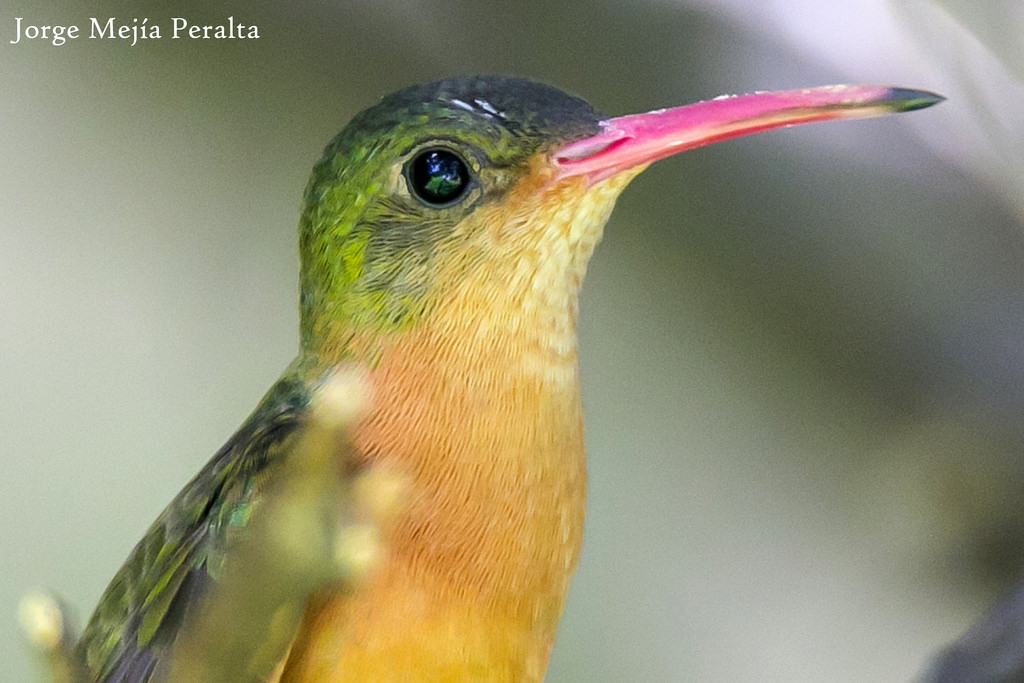
\includegraphics[width=.2\textwidth]{figures/chap3/crap/6}}}
    \subfigure{{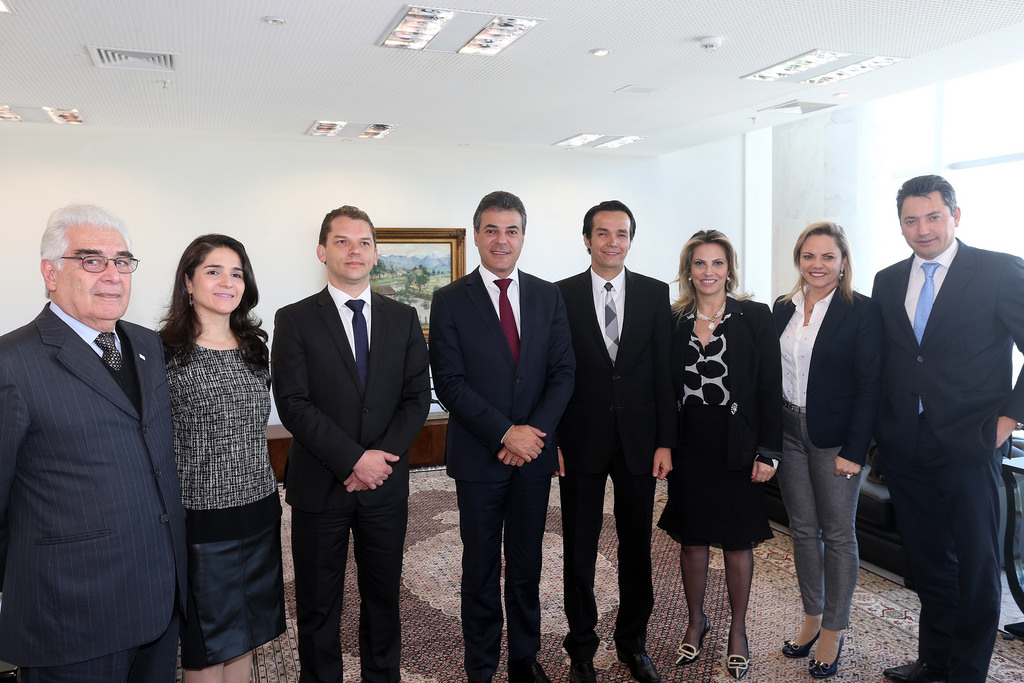
\includegraphics[width=.2\textwidth]{figures/chap3/crap/7}}}
    \subfigure{{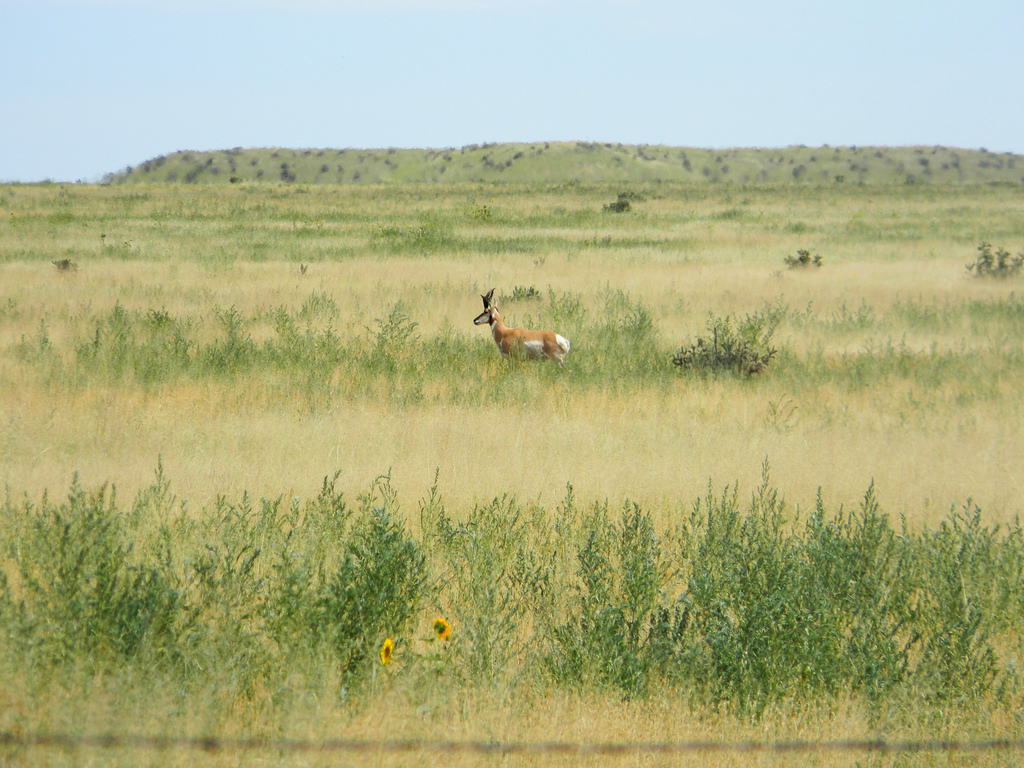
\includegraphics[width=.2\textwidth]{figures/chap3/crap/8}}}
    \caption{Sample figures from AADB dataset}
    \label{c3:crap}
\end{figure}

\begin{figure}[ht!]
    \centering  
    \subfigure[Images ranked the highest in aesthetics by DCNN]{{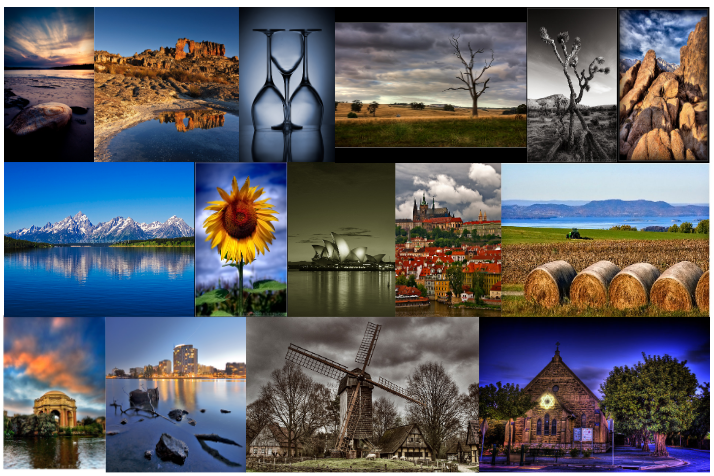
\includegraphics[width=.5\textwidth]{figures/chap3/crap/ava_good}}}
    \subfigure[Images ranked the lowest in aesthetics by DCNN]{{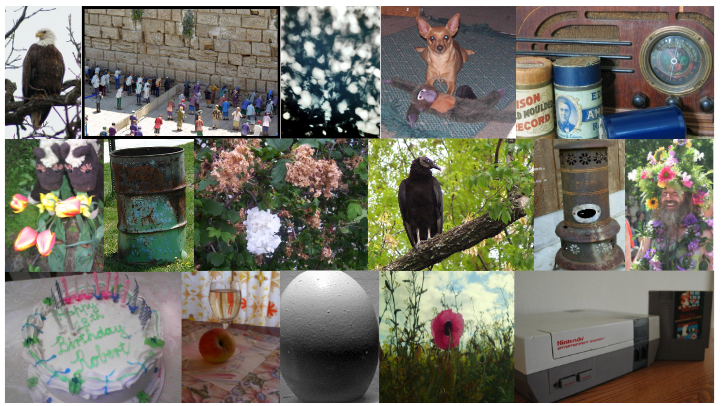
\includegraphics[width=.5\textwidth]{figures/chap3/crap/ava_crap}}}
    \caption{RAPID system, Lu et al. 2014~\cite{lu2014rapid}}
    \label{c3:ava_crap}
\end{figure}    
    
In the next Chapter, we present a recently published high competent data set, with super high resolution images, from Unsplash, a famous image sharing and publishing platform, adopted by famous products and web applications across industry.


%%%%%%%%%%%%%%%%%%%%%%%%%%%%%%%%%%%%%%%%%

\section{Active Learning}

In the latest decade, deep learning models have achieved groundbreaking results on several computer vision tasks~\cite{he2015delving},~\cite{krizhevsky2012imagenet},~\cite{he2016deep} and have become very popular due to their high flexibility, capacity and accuracy. Yet these models rely on vast amounts of labelled data for training. In practice, in many applications, we might not have access to such large data pools and more specifically we cannot afford to annotate all of them. Data labelling is an expensive and tedious task that is performed under a limited time budget, in addition the acquisition of a large number of high-quality annotated samples consumes a lot of manpower, making it unfeasible in fields that require high levels of expertise.

However, if there was an algorithm, that had the ability to suggest the samples from which it learns, it would achieve greater accuracy with less annotations.

%What will happen if we keep the model's hyperparameters and architecture fixed and experiment on different versions of data?

The paradigm of choosing the most informative data to label is referred to as \textit{active learning}~\cite{cohn1996active},~\cite{settles2009active}. The key challenge remains that there isn't any standardized method to determine the informativeness of the data. Active learning is performed in the context of sequential decision making where at every step, two operations are performed: i) measure the informativeness of the unlabelled data w.r.t. an active learner and choose the most informative to annotate, ii) update the underlying training data set with the new annotations and the active learner w.r.t. to the training performance.

Active learning is a training strategy, that aims to select the most beneficial samples from the unlabelled data set and send them to the oracle(human annotator) for labelling, in order to reduce the cost of labelling as much as possible while achieving high performance.

There are several \textit{scenarios} which an active learner can utilise and pose queries and several \textit{query strategies} that can been used to decide which instances are most informative.

\subsection{Active learning scenarios}

In random selection or in regular ``passive'' learning, the process is straightforward and new samples are chosen to get labelled uniformly from an unlabelled pool.

When employing an active learning scenario, we ask the active learner from a pool of unlabelled instances, to indicate the most informative samples that when included in training set will be more beneficial and perform better, in less training rounds, comparing to when trained with randomly selected samples.

Such active learning scenarios are considered the i) \textbf{Membership query synthesis}, ii)\textbf{Stream-based selective sampling} and iii) \textbf{Pool-based active learning}~\cite{settles2009active}, but only some of them can apply to our case study.

Membership query synthesis means that the learner can request to query the label of any unlabelled sample in the input space while in stream-based sampling, an independent judgement is made from the learner, on whether each sample in the data set is considered for annotation. The latter is rather the most expensive comparing to other methods as an additional mechanism is needed for the learner to decide if the candidate sample belong to the underlying distribution.

In pool-based scenario, unlabelled instances are selectively drawn from the pool and are typically queried in a greedy fashion, according to an informativeness measure used to evaluate all instances in the pool.

Applying the first scenario to our case study when querying from the pool of unlabelled instances the unexpected problem we encountered is that many of the query images generated were not contain any semantic meaning about the certain photography style (shallow/deep depth of field). 

Pool-based seems that applies better to our case study and based on an informativeness measure we can generate actively selected samples. In order to tackle the encountered problem, inspired from the second scenario, during the process of annotation, the problematic candidate samples where discarded from the selection. Finally we constructed a closed data set pool in order to apply the pool-based scenario.

Figure~\ref{c3:fig_pool_based} illustrates the framework diagram from pool based strategy. To initialise the process(bootstrap), we can select randomly samples from unlabelled pool \textit{U}, obtain labels in order to generate a labelled training set \textit{L} and train a machine learning model \textit{C}. Next, we use this model as an active learner, by applying a query strategy framework in order to select the next annotated samples. The process is repeated until the label budget is exhausted or the termination conditions are met(e.g. data depletion, query strategy limits).

\begin{figure}[ht!]
    \centering  
    {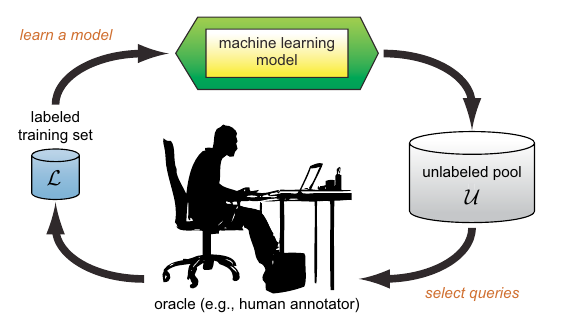
\includegraphics[width=.5\textwidth]{figures/chap3/active_learning/pool_based}}
    \caption{Pool based active learning}
    \label{c3:fig_pool_based}
\end{figure} 

\subsection{Query strategy framework}

The simplest and most commonly used query framework is uncertainty sampling, where an active learner queries the samples that it can predict with least confidence (LC)~\cite{settles2009active}. Those samples are considered as the most informative ones or the most ambiguous, as the classifier is uncertain for the predicted class. This of course requires the use of a model that is capable of assessing adequately the prediction uncertainty.

The aforementioned query strategy when applied in DAL can be implemented with the output of the softmax layer of the deep learned classifier, thus the query strategy based on uncertainty is widely used in a variety of studies~\cite{ren2020survey}.

For this reason, Deep Bayesian Active Learning (DBAL)~\cite{gal2017deep} has been developed. For a given input set $\text{X}$ and the network output $\text{Y}$ belonging to class, the probabilistic neural network can be defined as $f(x;\theta), p(\theta)$ is a prior on the parameter space $\theta$, and the likelihood $p(y = c|x,\theta)$ is usually determined by $\text{softmax}(f(x;\theta))$. The goal is to obtain a posterior distribution over $\theta$, as follows:

\begin{ceqn}
\begin{align}
    p(\theta|X,Y) = \frac{p(Y|X, \theta)p(\theta)}{p(Y|X)}
\end{align}  
\end{ceqn}

For a new given(inferenced) observation $x^*$, a $\hat{y}$ prediction is made:

\begin{ceqn}
\begin{align}
    p(\hat{y}|x^*, X, Y) = \int p(\hat{y}|x,\theta) p(\theta|X, Y)d\theta
\end{align}  
\end{ceqn}

Thus, least confidence(LC) measurement is given from:

\begin{ceqn}
\begin{align}
     x_{LC}^{*} = argmin_{x} P( \hat{y} | x;\theta ) 
\end{align}  
\end{ceqn}

where $\hat{y} = \text{argmax}_y P(\hat{y}|x;\theta)$, is the most likely predicted class. 

Hence, we use the probabilities as indicators of classification uncertainty.


\subsection{Batch-Mode Deep Active learning}
\label{c5:section_batch_mode_learning}
Formulating the above, we are looking for these samples that will be selected from the active learner, transferred systematically to a human annotator(oracle) and consequently will returned back to the training set, get the model retrained and so forth, achieve better classification performance.

In most active learning research, queries are selected in serial, e.g. one at a time. For the context of DL, the one-by-one sample query method which commonly used in AL is not applicable.
Consider also that sometimes a distributed, parallel labelling environment may be available, e.g. labels are obtained from multiple annotators at the same time.

Selecting queries in serial may be inefficient and in contrast, \textit{batch-mode} active learning allows the learner to query instances in batches which resembles a parallel labelling practice or models with slow training procedures~\cite{settles2009active}.


Moreover, many ML algorithms don't re-train sequentially or retraining does not provide a statistically significant impact on the model, as is the case for many DL models.
In addition, this query method is not only inefficient in the training of the DL model, but can also easily lead to overfit~\cite{zhdanov2019diverse}.

Although there is not any standard rule to determine the number of batches that can be used to an active learning experiment there are works that compare and assess multiple volumes of active batches~\cite{gissin2019discriminative}. In this thesis we choose to experiment in two options. One with variable size of batch without incremental training and an option with a standard batch size of 100 samples and incremental training.


\subsection{Deep Active Learning}

DL has demonstrated abilities to process high-dimensional data though the automated feature extraction mechanisms, while AL has substantial potential to reduce annotation costs. Therefore, combining the two approaches, will effectively benefit the applications performance.

Recent studies and developments in Deep and Active learning are transitioning from the model-centric to the emerging field of data-centric artificial intelligence~\cite{bosser2020model},~\cite{motamedi2021datacentric} which is expected to deliver techniques for data set optimization, thereby to more efficient training with less samples and annotations. 

This falls into an active learning framework with deep learning, known as deep active learning (DAL), that will be able to select the most informative samples, send them to an oracle for annotation and append them to the data set, as it is shown in Figure~\ref{c4:fig_al_procedure}.

\begin{figure}[ht!]
    \centering  
    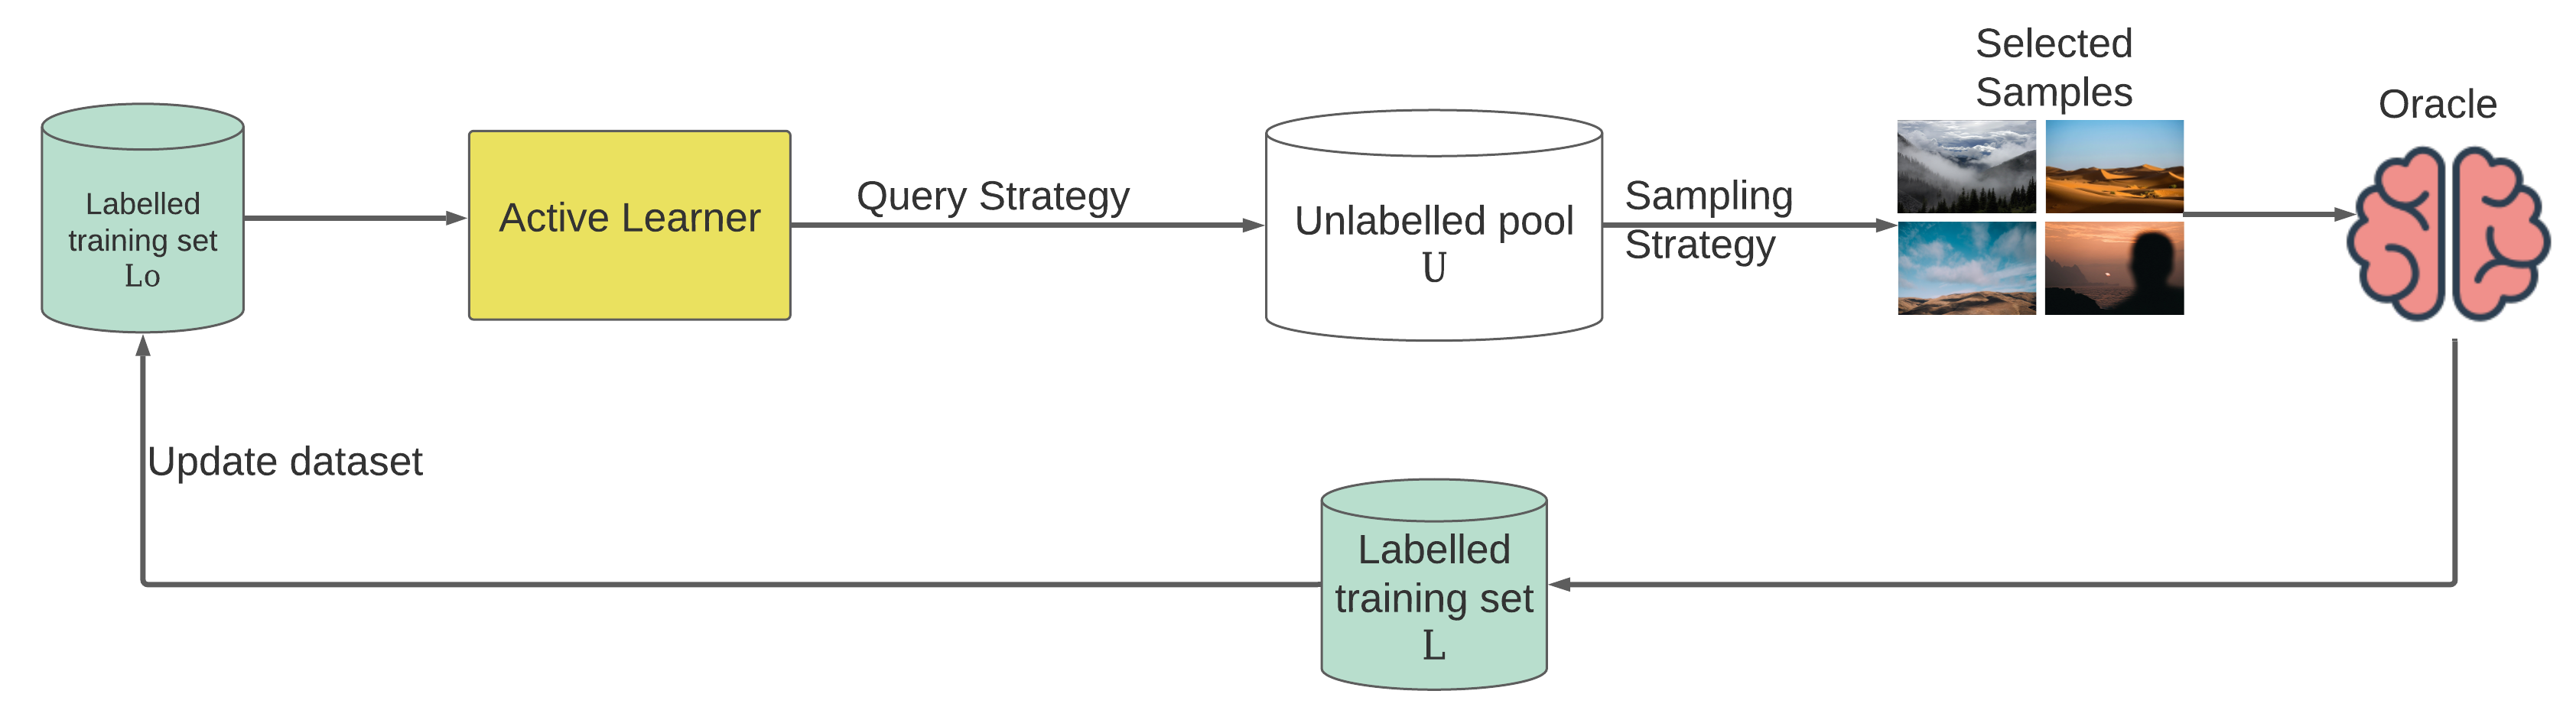
\includegraphics[width=\textwidth]{figures/chap5/al/al_map}
    \caption{A typical example of DAL: A DL model is pre-trained on the labelled training set \textit{$L_0$}, and given a query strategy is used to select the next samples from the Unlabelled pool \textit{U}. A sampling strategy is to pick the candidate images and they are sent to a human oracle for annotation. The new labelled training set \textit{L} updates the initial \textit{$L_0$} and retrains the Deep Learning model.}
    \label{c4:fig_al_procedure}
\end{figure}

However, we have to consider two things. Deep learning poses several difficulties when used in an active learning setting. First, we have to be able to handle small amounts of data, yet recent developments in deep learning require large amounts of data~\cite{krizhevsky2009learning},~\cite{krizhevsky2012imagenet}. Second, many AL strategies rely on prediction uncertainty and such a case is rare in deep learning~\cite{gal2017deep}.
Concerning the latter, there are studies~\cite{wang2014new},~\cite{wang2016cost} that pose an unreliability to softmax when used to estimate the informativeness of the unlabelled samples and argue that the results may be worse than random selection.

In this thesis, we are studying a challenging and non trivial task thus we will follow the simplest approach using DBAL to exploit an active learning indicator and consequently implement and active learning algorithm.

Active learning using deep learning aims to achieve the best learning result given a limited labelled data set. Given a budget on the available unlabelled instances to have them annotated, our objective is to maximize the classifier's performance with the less cost effective method.

At each iteration, an active learning algorithm has two stages: a) identify a set of unlabelled instances and send them to a human oracle for annotation; and b) train a classifier using both the new and the previously labelled instances. The second stage (train the classifier) can be done in a fully or weakly-supervised manner. 
Fully-supervised is the case when the classifier is trained using only human labelled instances. Weakly-supervised is the case where training runtime utilise the points which are not labelled yet. Although the existing literature focuses most on the active learning for fully-supervised models, we consider both cases in our experiments.


\subsection{Cost Effective Active Learning (CEAL)}
\label{c5:section_ceal}

Another technique different from the existing AL approaches that consider only the most informative samples to get labelled from a human annotator, is one that poses the most confident queried unlabelled samples and automatically pseudo-annotates them without active user labelling.
Samples queried to an active learner with high predicted confidence are the most certain to get classified correctly. The method that selects these samples and automatically assign the predicted class as a pseudolabel, with any human labor cost, is proposed as cost-effective active learning (CEAL)~\cite{wang2016cost}. Figure~\ref{c5:figure_ceal} illustrates the method.

\begin{figure}[ht!]
    \centering  
    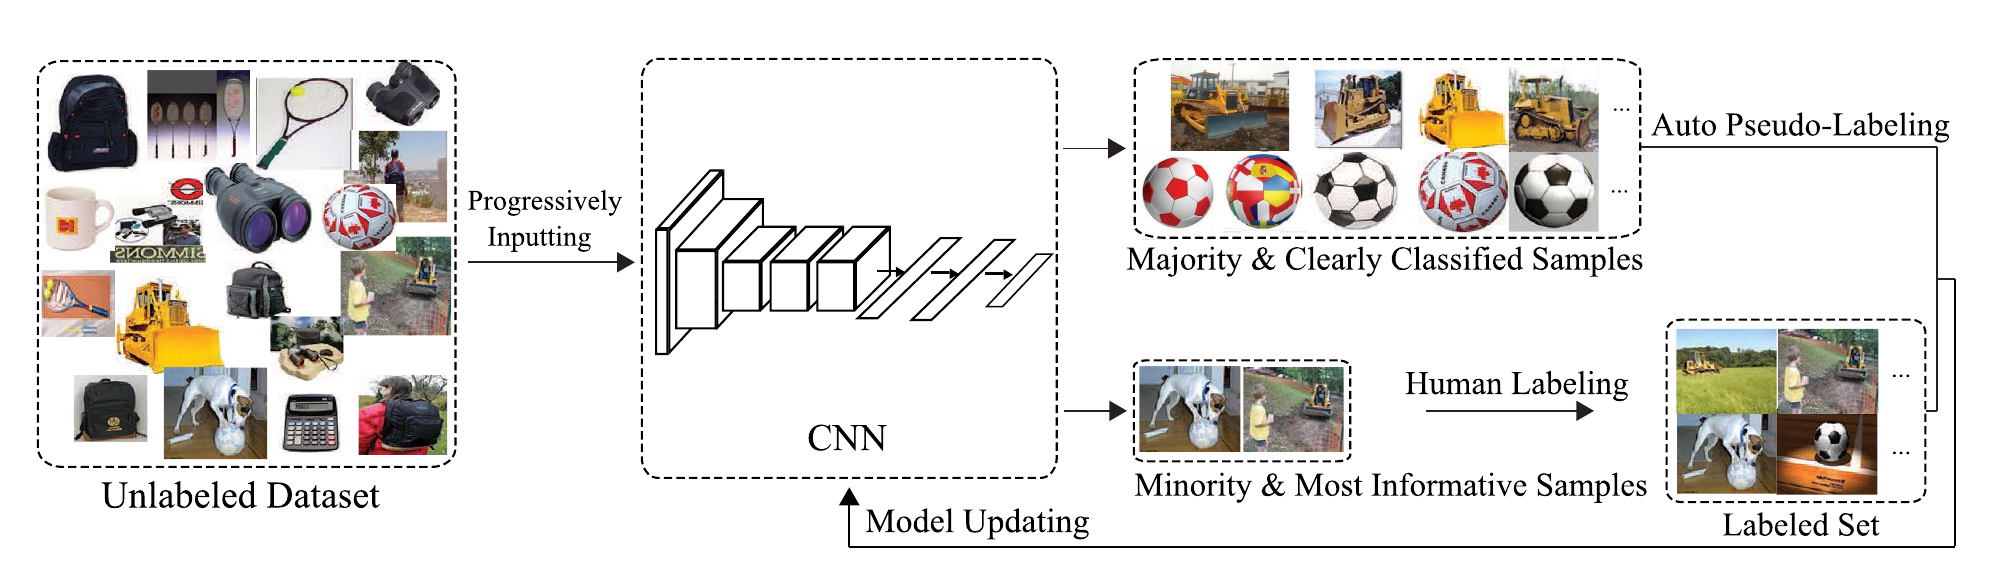
\includegraphics[width=\textwidth]{figures/chap5/al/ceal}
    \caption{CEAL progressively feeds the samples from the unlabelled data set into the CNN. The clearly classified samples are pseudolabelled while the most uncertain are send to manual annotation.}
    \label{c5:figure_ceal}
\end{figure}


\subsection{Cached Annotation Batch-Mode Active learning}
\label{c5:section_cached_setting}

Following a closed loop strategy, similar to the Figure~\ref{c4:fig_al_procedure}, it requires the model to be retrained on the whole labelled data set, once new labels are available. For very large modern deep CNN's that require many hours of end-to-end training, this is typically impractical.

% prepei na koitame kai thn pragmatistiki plevra toy provlimatos kai oxi mono tin ideati
In practice, this scenario is often unrealistic: in order to be able to implement such a loop in a production environment the budget for human annotations is limited or might be a deterring factor to construct a fully automated pipeline.
Also the AL strategy has to be closely integrated with the annotation system, something that may introduce limits to the data owner.

In this work, inspired from pool based and batch-mode strategies, we have combined and evaluated both methods in two different active learning settings, that we present in Section~\ref{c5:section_experimental_setup}.

The intuition behind both settings is that they do not adhere in a closed training-query-annotation loop, thus do not require to ask or wait for new labels. All queried ``unlabelled'' samples have been annotated once (pre-annotated) given a time budget. This practice enables the machine learning practitioner to construct a fully automated pipeline without waiting for unlabelled samples to get labelled, instead the active learning algorithm can be designed on what samples will pick next.

We create a new setting of ``caching'' the annotations and named it after ``Cached Annotation Batch-Mode Active Learning''. 
A closed sampling pool is comprised from randomly and actively selected samples, with ``cached'' annotations obtained once at the bootstrap step.

More specifically in Section~\ref{c5:section_al_simulation} we apply a simulation algorithm with \textbf{single} and \textbf{increamentally} trained active learners, on the same pool of pre-annotated samples and demonstrate random and active selection strategies, without asking for extra annotations.
